
\chapter{Background Estimation and Validation}
\label{bg_val}
\section{Introduction}
This chapter describes the techniques used for estimation of the backgrounds in the analyses. Each background is estimated individually. For large backgrounds, the estimation is validated using regions enriched in those backgrounds.

\section{\hmue backgrounds}
\label{h125_bg_val}

\subsection{\ztt}
\label{h125_ztt}
The \ztt background is the dominant background in 0-jet and 1-jet categories of the analysis. It is an irreducible background and arises when one $\Pgt$ coming from the $\PZ$ boson decay further decays into a $\Pgm$ and the other decays into a $\Pe$. This background is estimated from simulated monte-carlo events. In a $\PZ \to \ell \ell$ events from Drell-Yan production including \ztt, the $m_{\ell\ell}$ and $\PZ_{\pt}$ distribution is found to be different in data and simulation. In order to correct for this, a set of reweighting factors is calculated using a dedicated control region enriched in $\PZ \to \Pgm\Pgm$ events. The set of reweighting factors are applied as a function of generator-level $m_{\ell\ell}$ and $\PZ_{\pt}$ in the signal region of the analysis. A more detailed study of this effect and calculation of the reweighting factors can be found in the following references~\cite{}.

To validate this estimation, we look at agreement between observed data and simulation in a region enriched in \ztt events. This region is constructed by requiring, in addition to the baseline selection,  the $\pt$ of the $\Pgm<40$ \GeV. The $\pt$ in \ztt events is on softer side of the spectrum compared to other backgrounds which are more spread out, as seen in Fig.~\ref{fig:h125_presel1} (top right). The $M_T(\Pgm)$, as seen in Fig.~\ref{fig:h125_presel1} (bottom right), is required to be less than 60\GeV following similar reasoning. Further the invariant mass of the $\Pe$ and $\Pgm$ is required to be in between 30\GeV and 70\GeV in order to isolate the $\PZ$ peak. The distributions of BDT response and \mcol in this \ztt enriched region are shown in Fig.~\ref{fig:ztt_cr}, for the categories where this background is dominant. The plots show good agreement between data and background.



\begin{figure*}[!htpb]\centering
 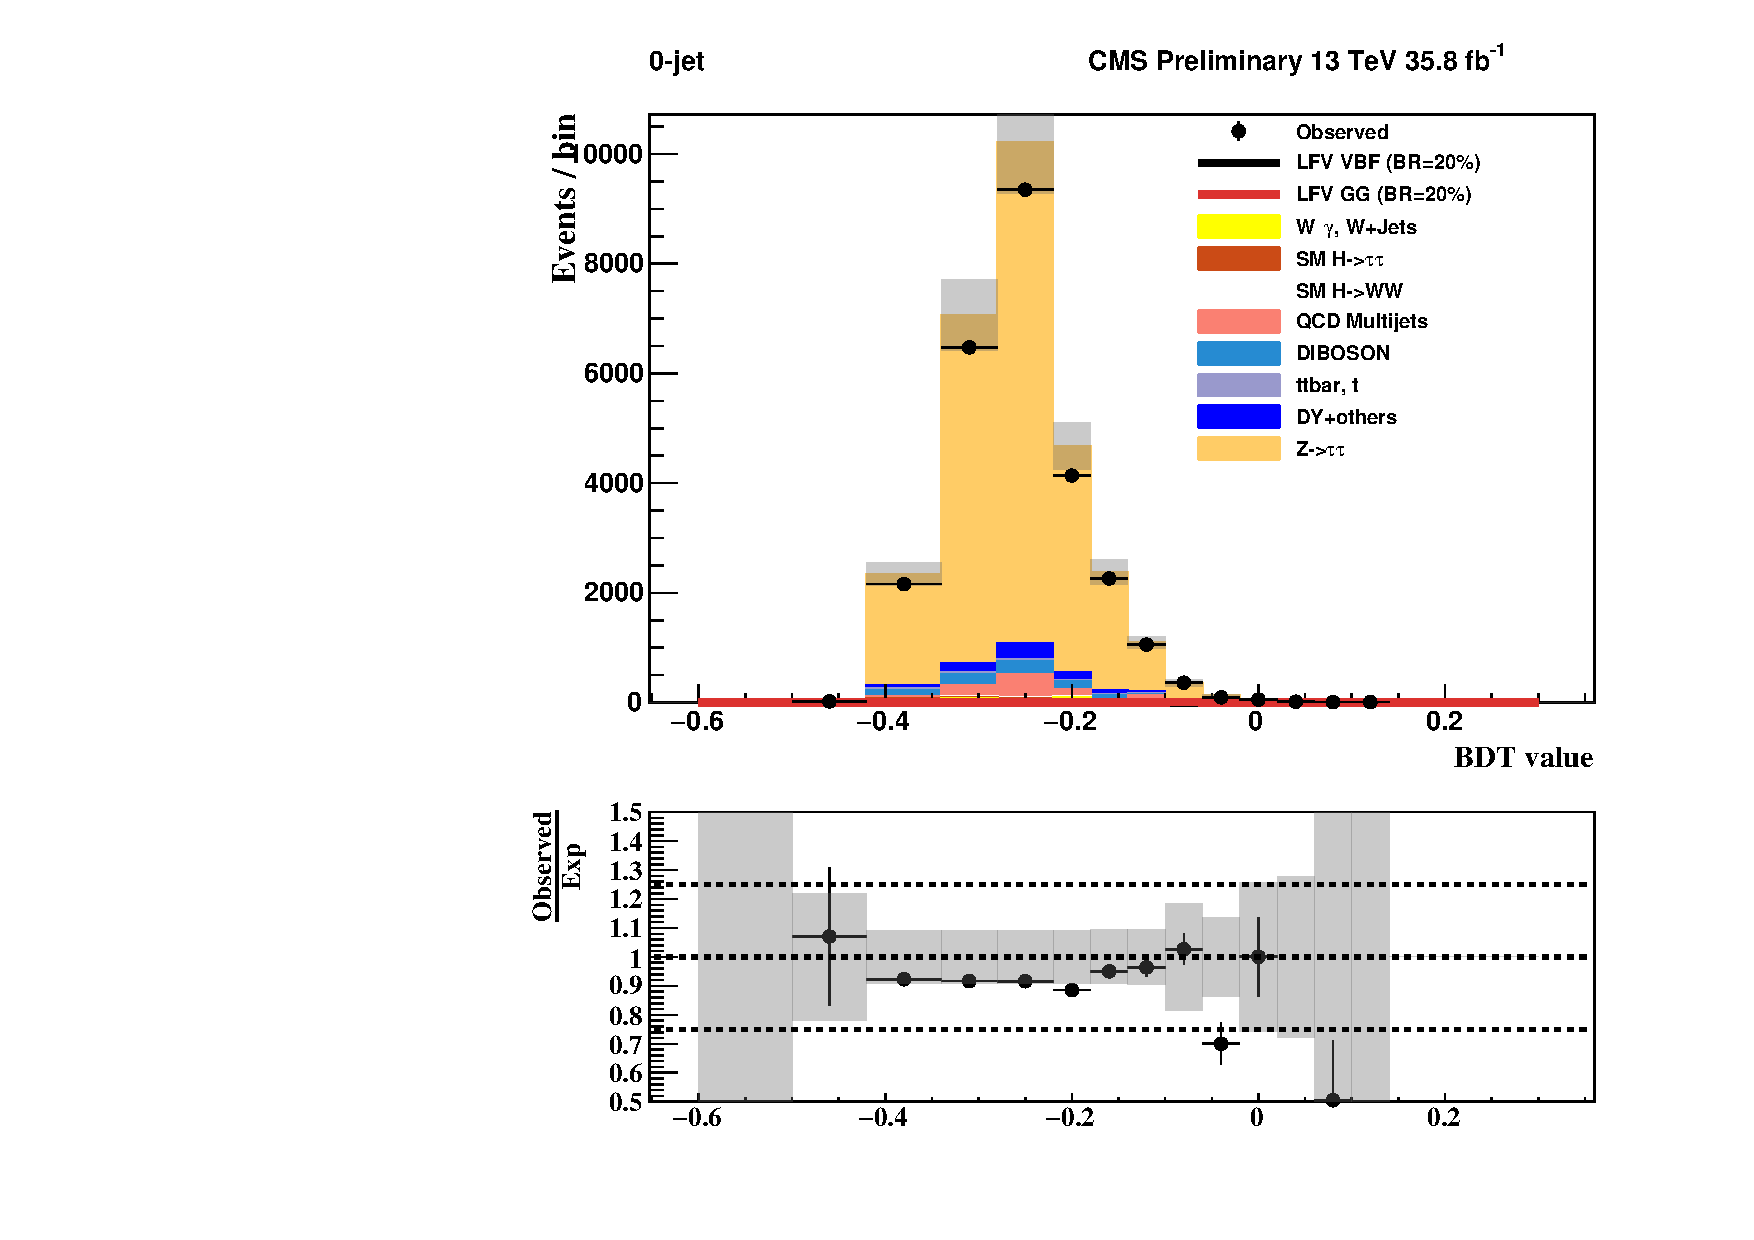
\includegraphics[width=0.49\textwidth]{plots_and_figures/chapter6/ztt_cr/0_preselection_BDT_value.pdf}
 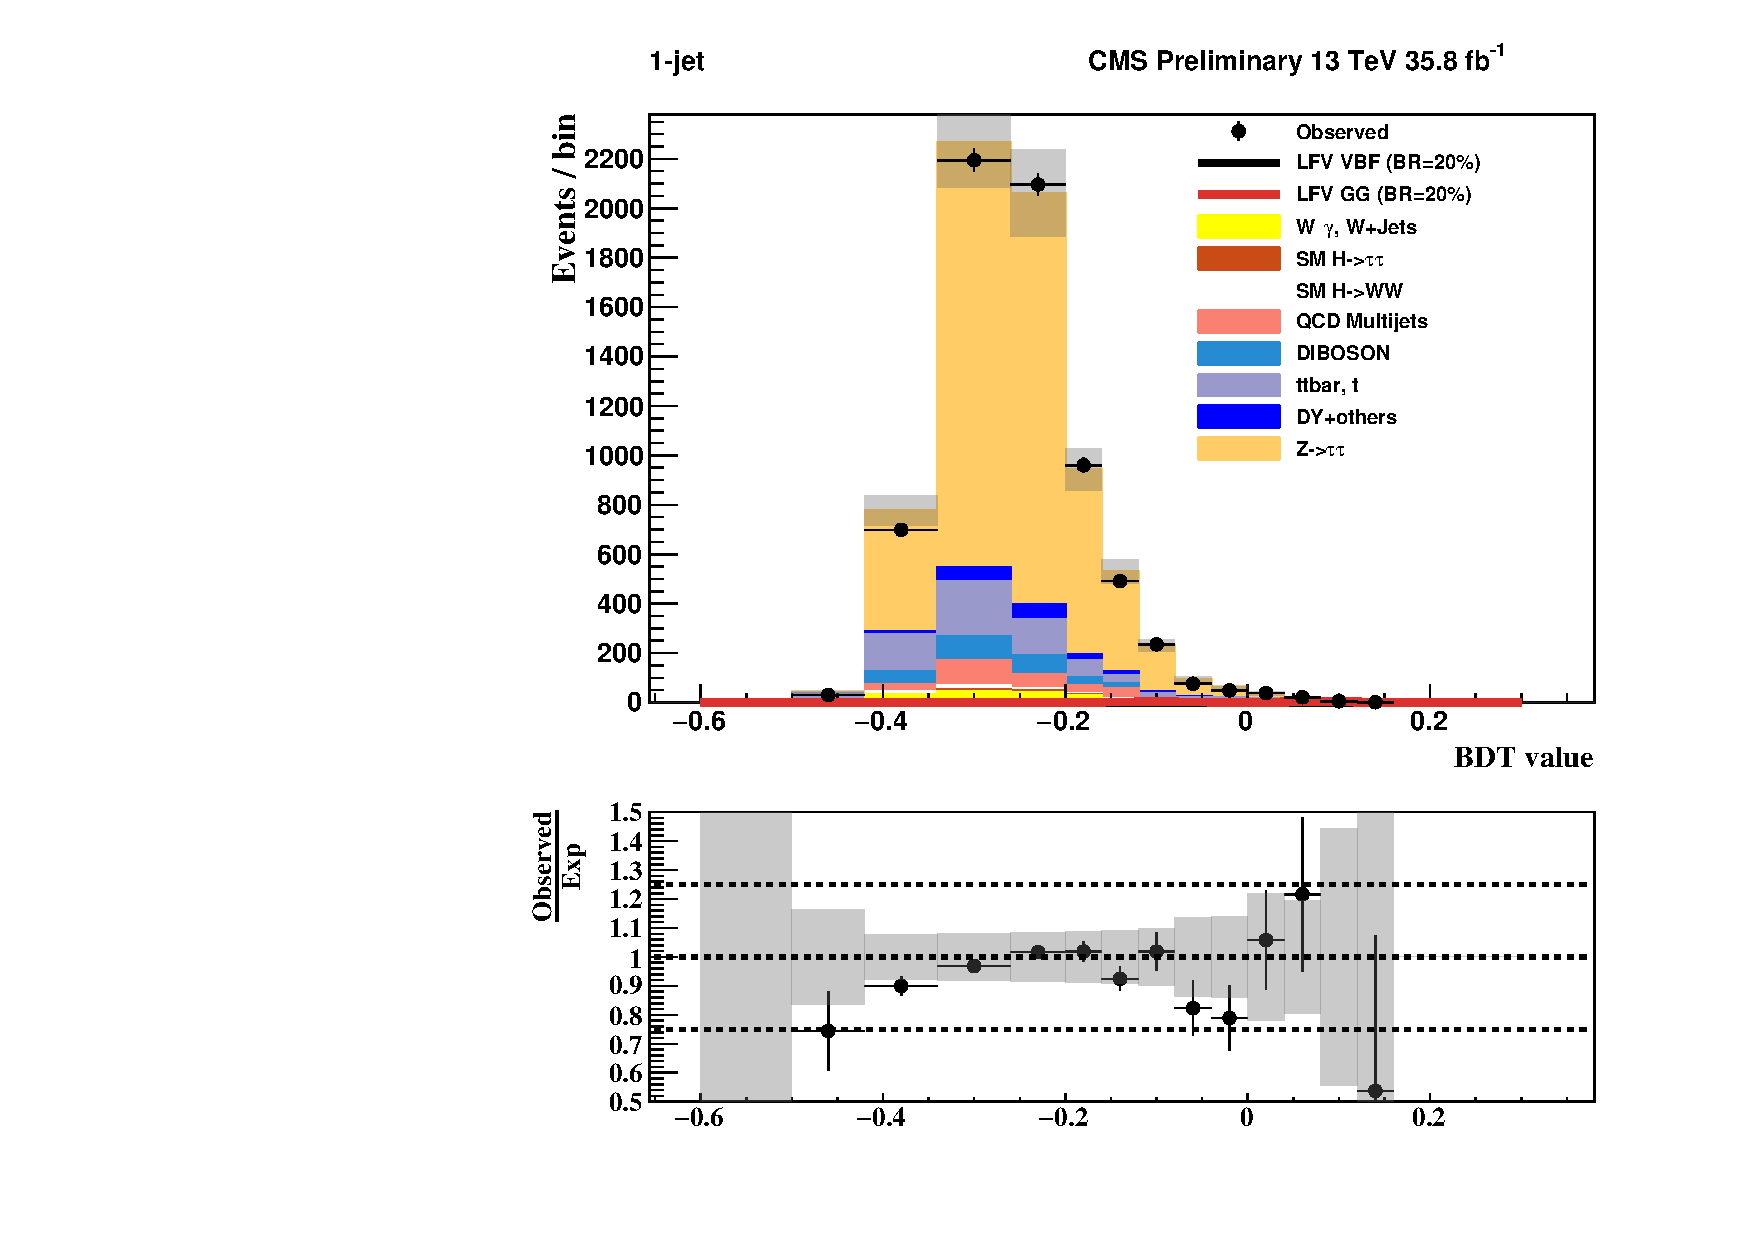
\includegraphics[width=0.49\textwidth]{plots_and_figures/chapter6/ztt_cr/1_preselection_BDT_value.pdf} \\
 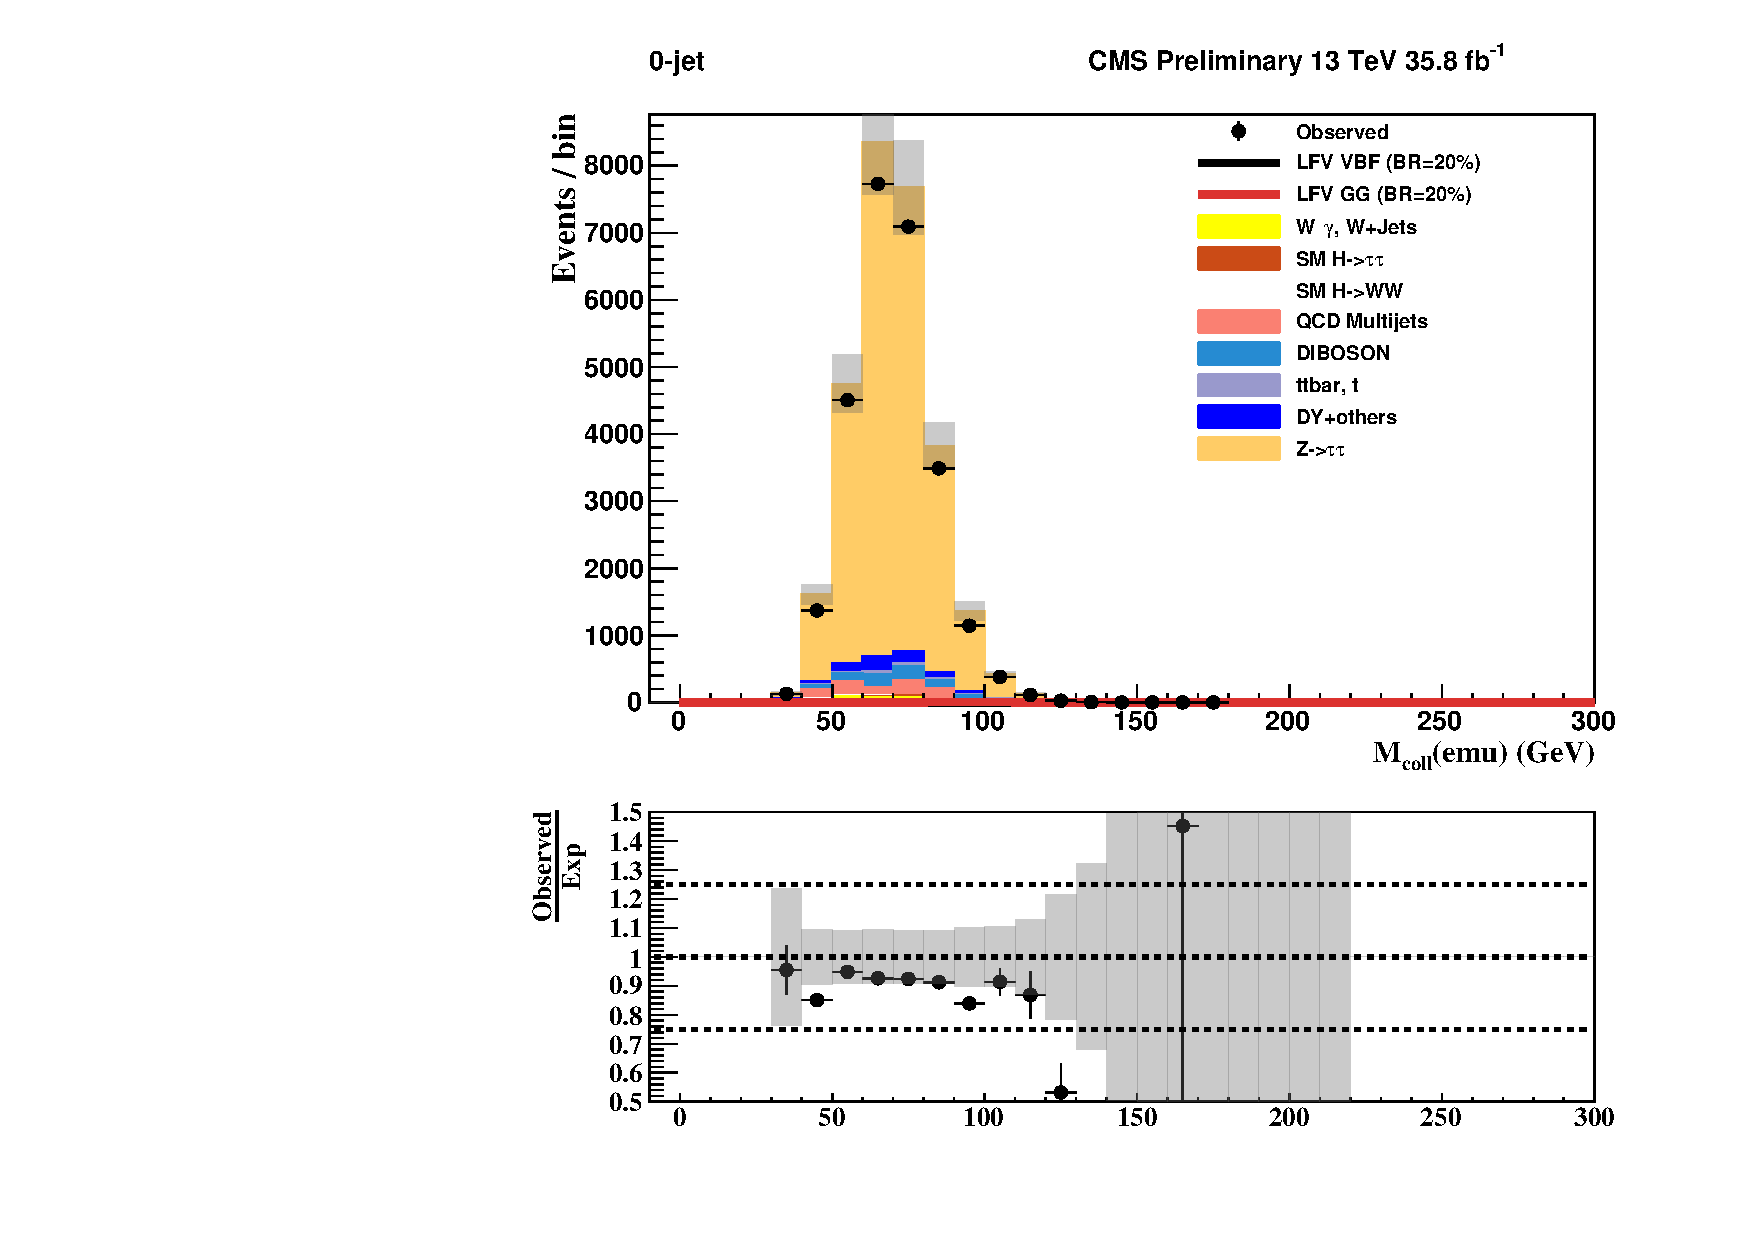
\includegraphics[width=0.49\textwidth]{plots_and_figures/chapter6/ztt_cr/0_preselection_h_collmass_pfmet.pdf} 
 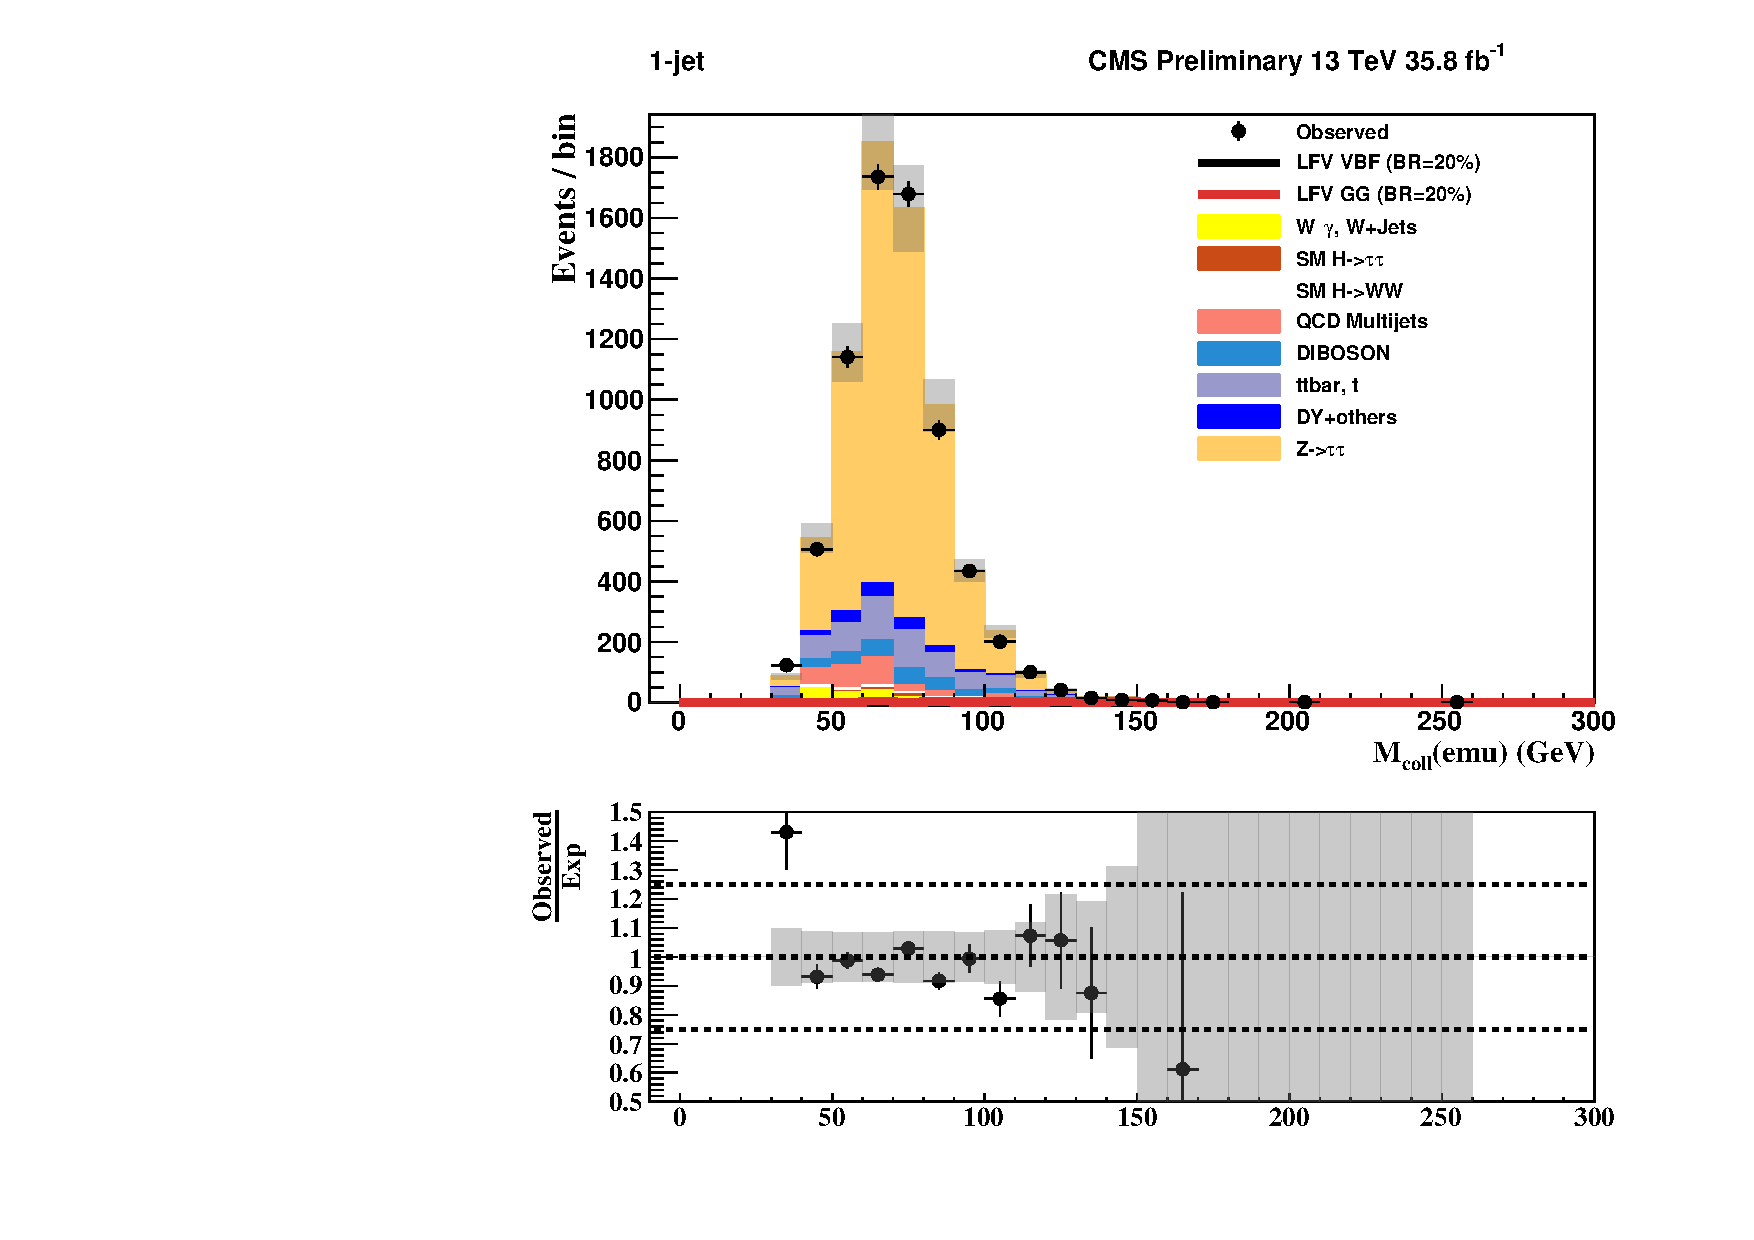
\includegraphics[width=0.49\textwidth]{plots_and_figures/chapter6/ztt_cr/1_preselection_h_collmass_pfmet.pdf} \\

 \caption{Distributions of BDT response (top) an \mcol (bottom) in \ztt enriched region for 0-jet (left)  and 1-jet (right) categories.}
 \label{fig:ztt_cr}
\end{figure*}


\subsection{\ttb}
\label{h125_ttb}
Tops decay into $\PW$ bosons and a b-quark more than 90\% of the time. The $\PW$ boson can decay leptonically into a $\Pgm$ and $\Pe$ making it a background for the analysis. The b-tagging veto applied at the baseline selection level is able to somewhat supress this background. However it still forms a large fraction of the background for the anlysis. In fact, it is the largest background in both 2-jet categories. It is also large in the 1-jet category. We estimate the \ttb background using simulation. The background estimation is validated in two separate control regions enriched in \ttb. The first control region is formed requiring the baseline selection but with a inverted b-tagging veto. In other words, at least 1 b-tagged jet is required to be present in the event. The distributions of BDT response (top) and \mcol (bottom) in this region are shown in Fig.~\ref{fig:tt_cr} for categories where the \ttb background is large. The second control region is constructed using kinematic selection criteria. In particular, in addition to the baseline selection criteria with the b-tag veto removed, we require $M_T(\Pe)$ (see Fig.~\ref{fig:h125_presel2} top left) to be greater than 50\GeV. The distributions of BDT response (top) and \mcol (bottom) in this second control region are shown in Fig.~\ref{fig:tt_cr_cutbased}. Given that the uncertainty bands in these control region plots only contain uncertainties on normalization (and not shape-based uncertainties, as discussed in section~\ref{sig_ext}, and included in the max likelihood fit used to extract results), the data over background estimation  ratio is reasonable in these regions. Further,a normalization uncertainty of 10\% is applied on the \ttb estimation in the signal region based on these control regions.


\begin{figure}[!htpb]\centering
 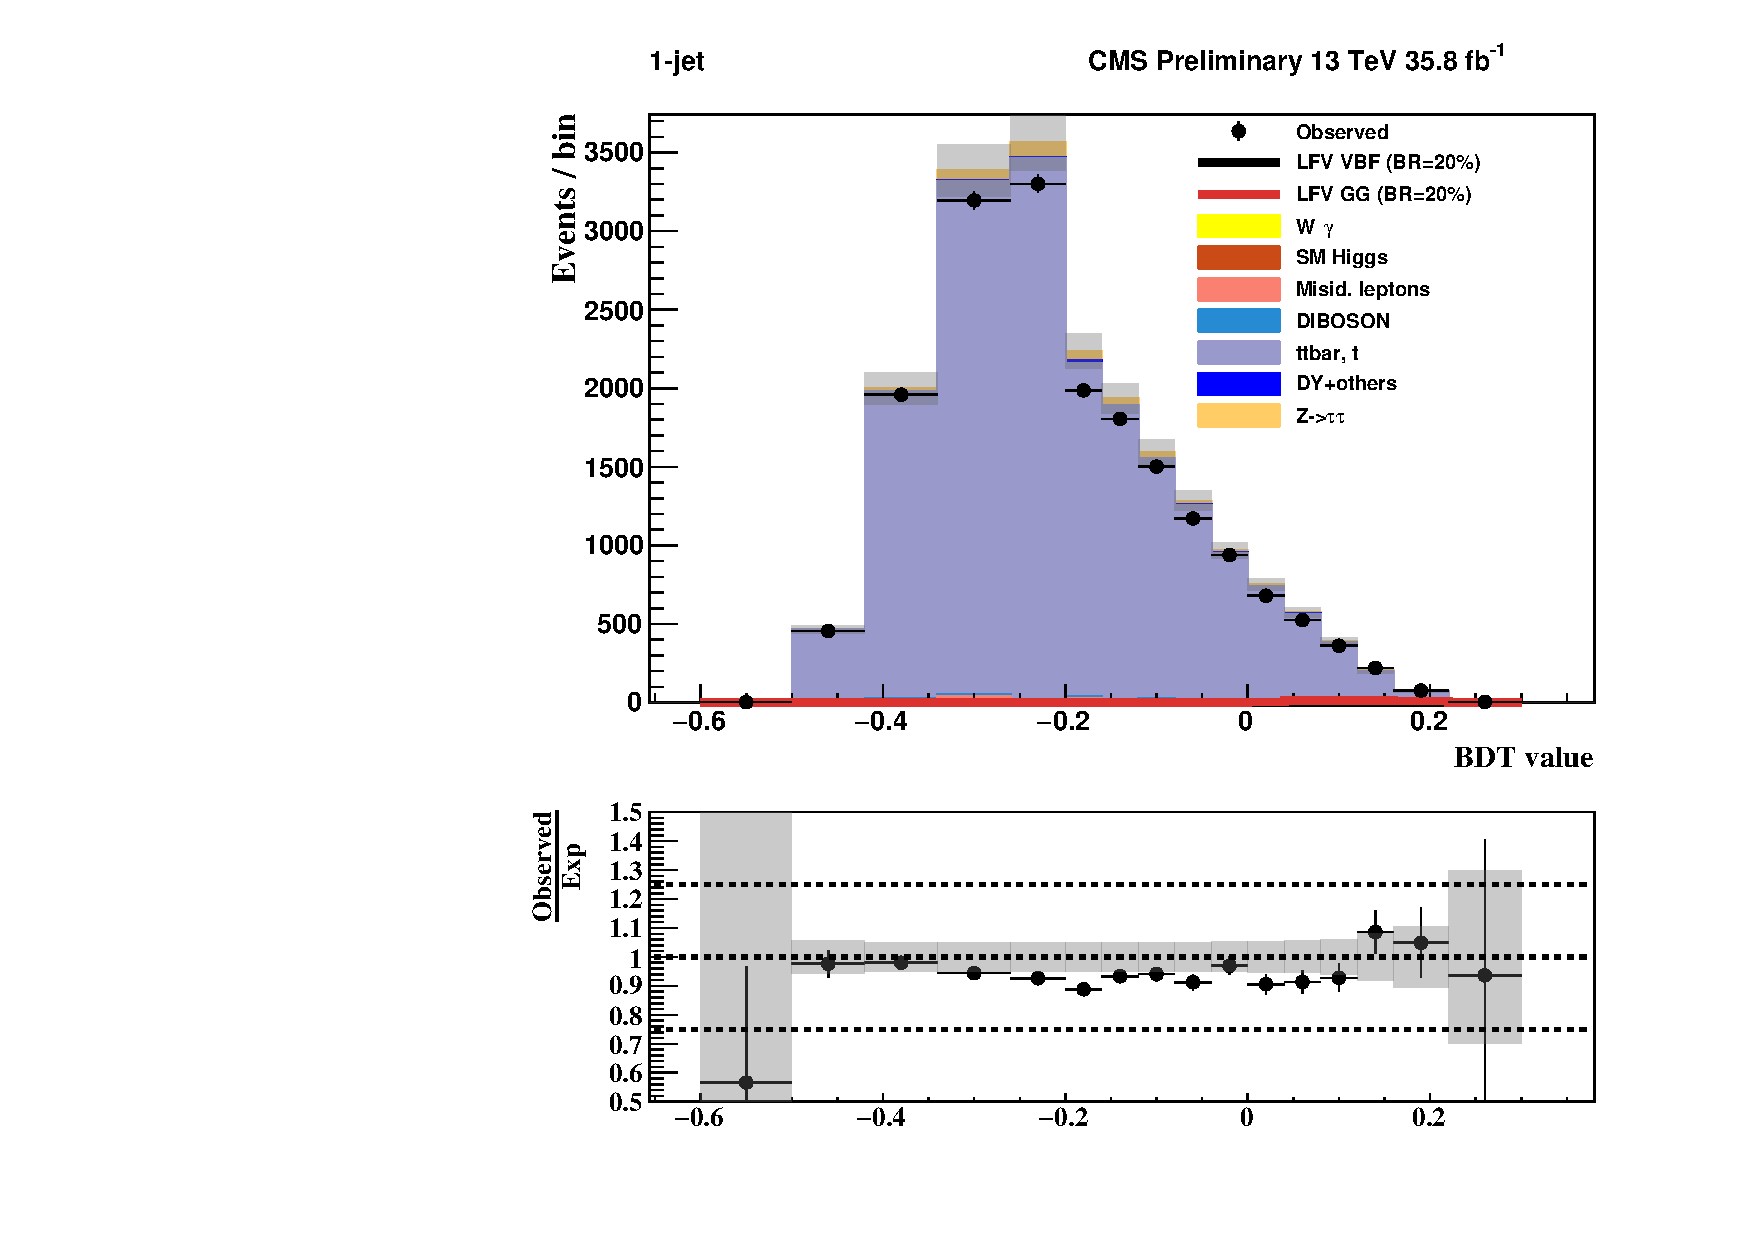
\includegraphics[width=0.30\textwidth]{plots_and_figures/chapter6/tt_cr/1_preselection_BDT_value.pdf}
 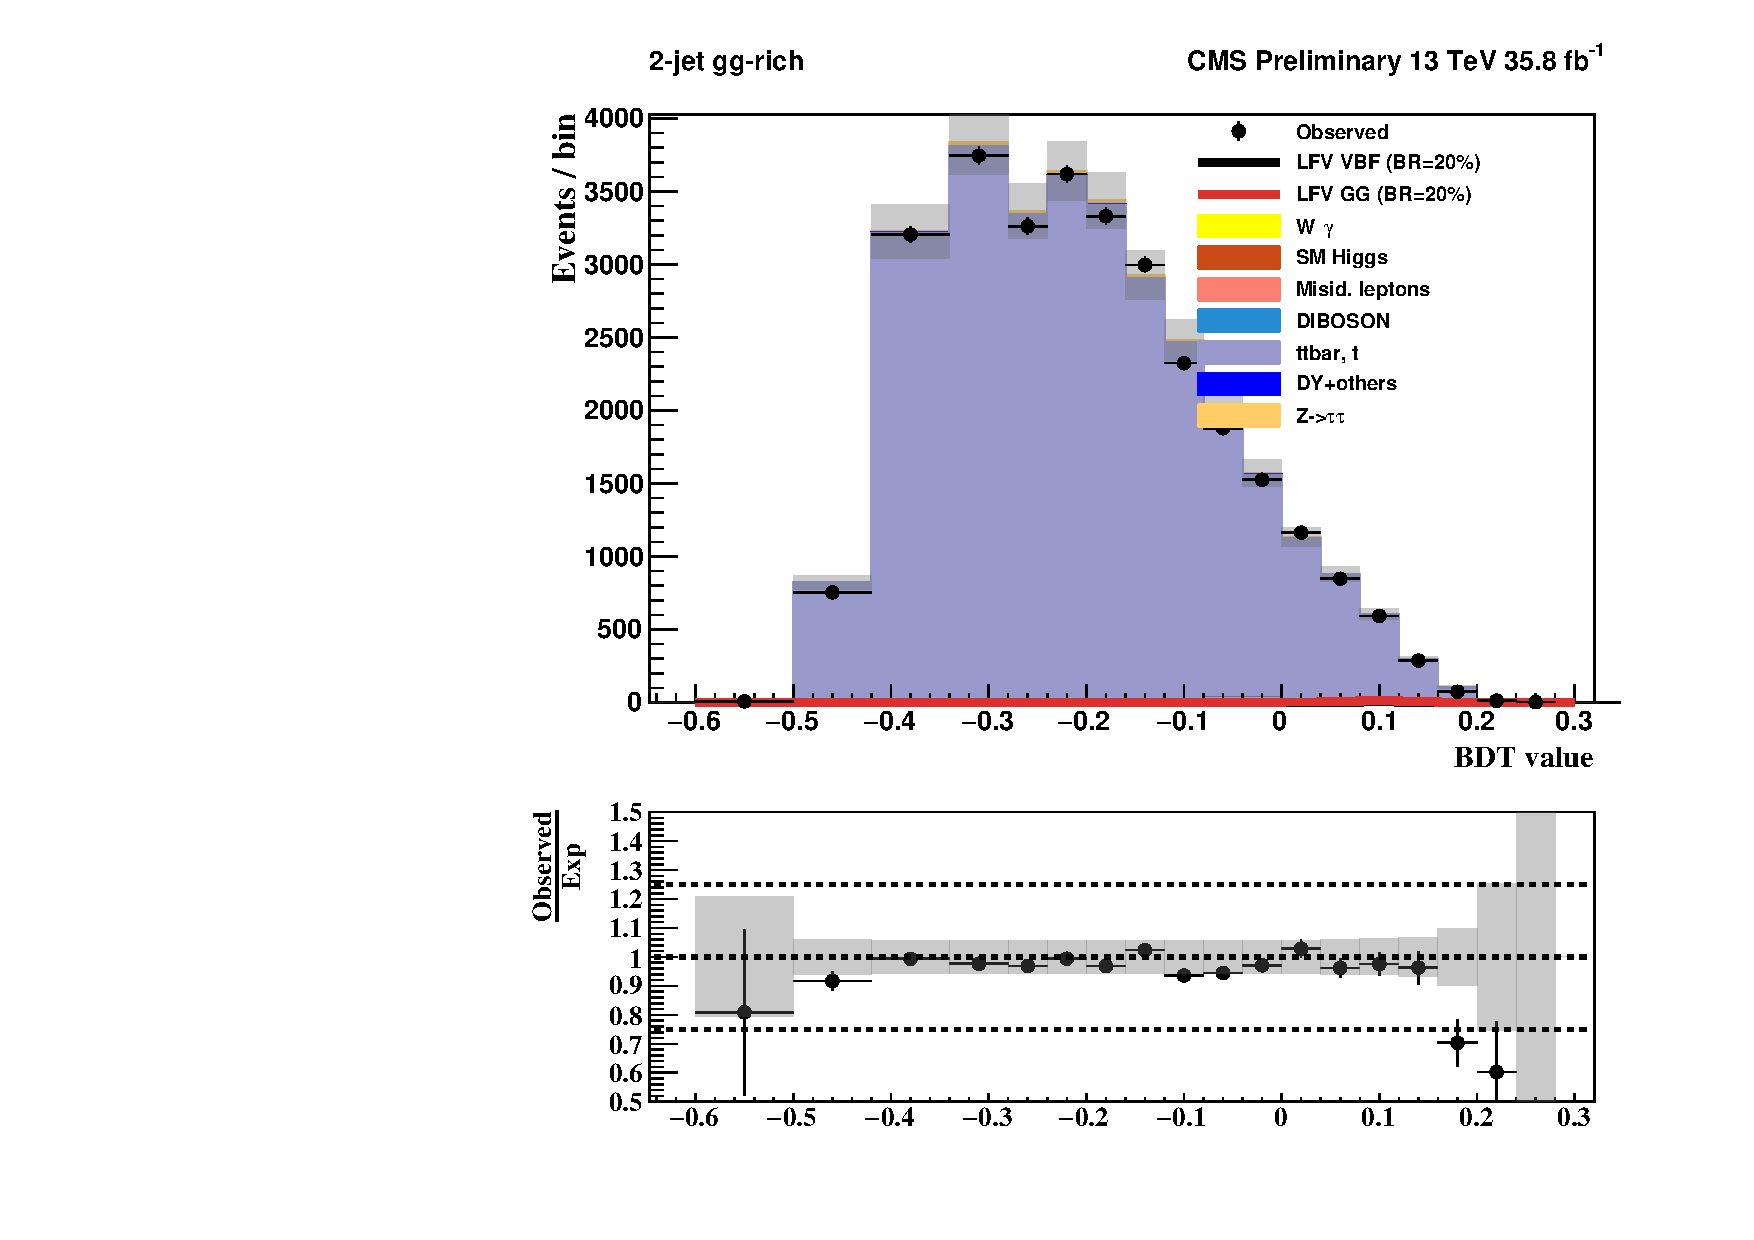
\includegraphics[width=0.30\textwidth]{plots_and_figures/chapter6/tt_cr/21_preselection_BDT_value.pdf} 
 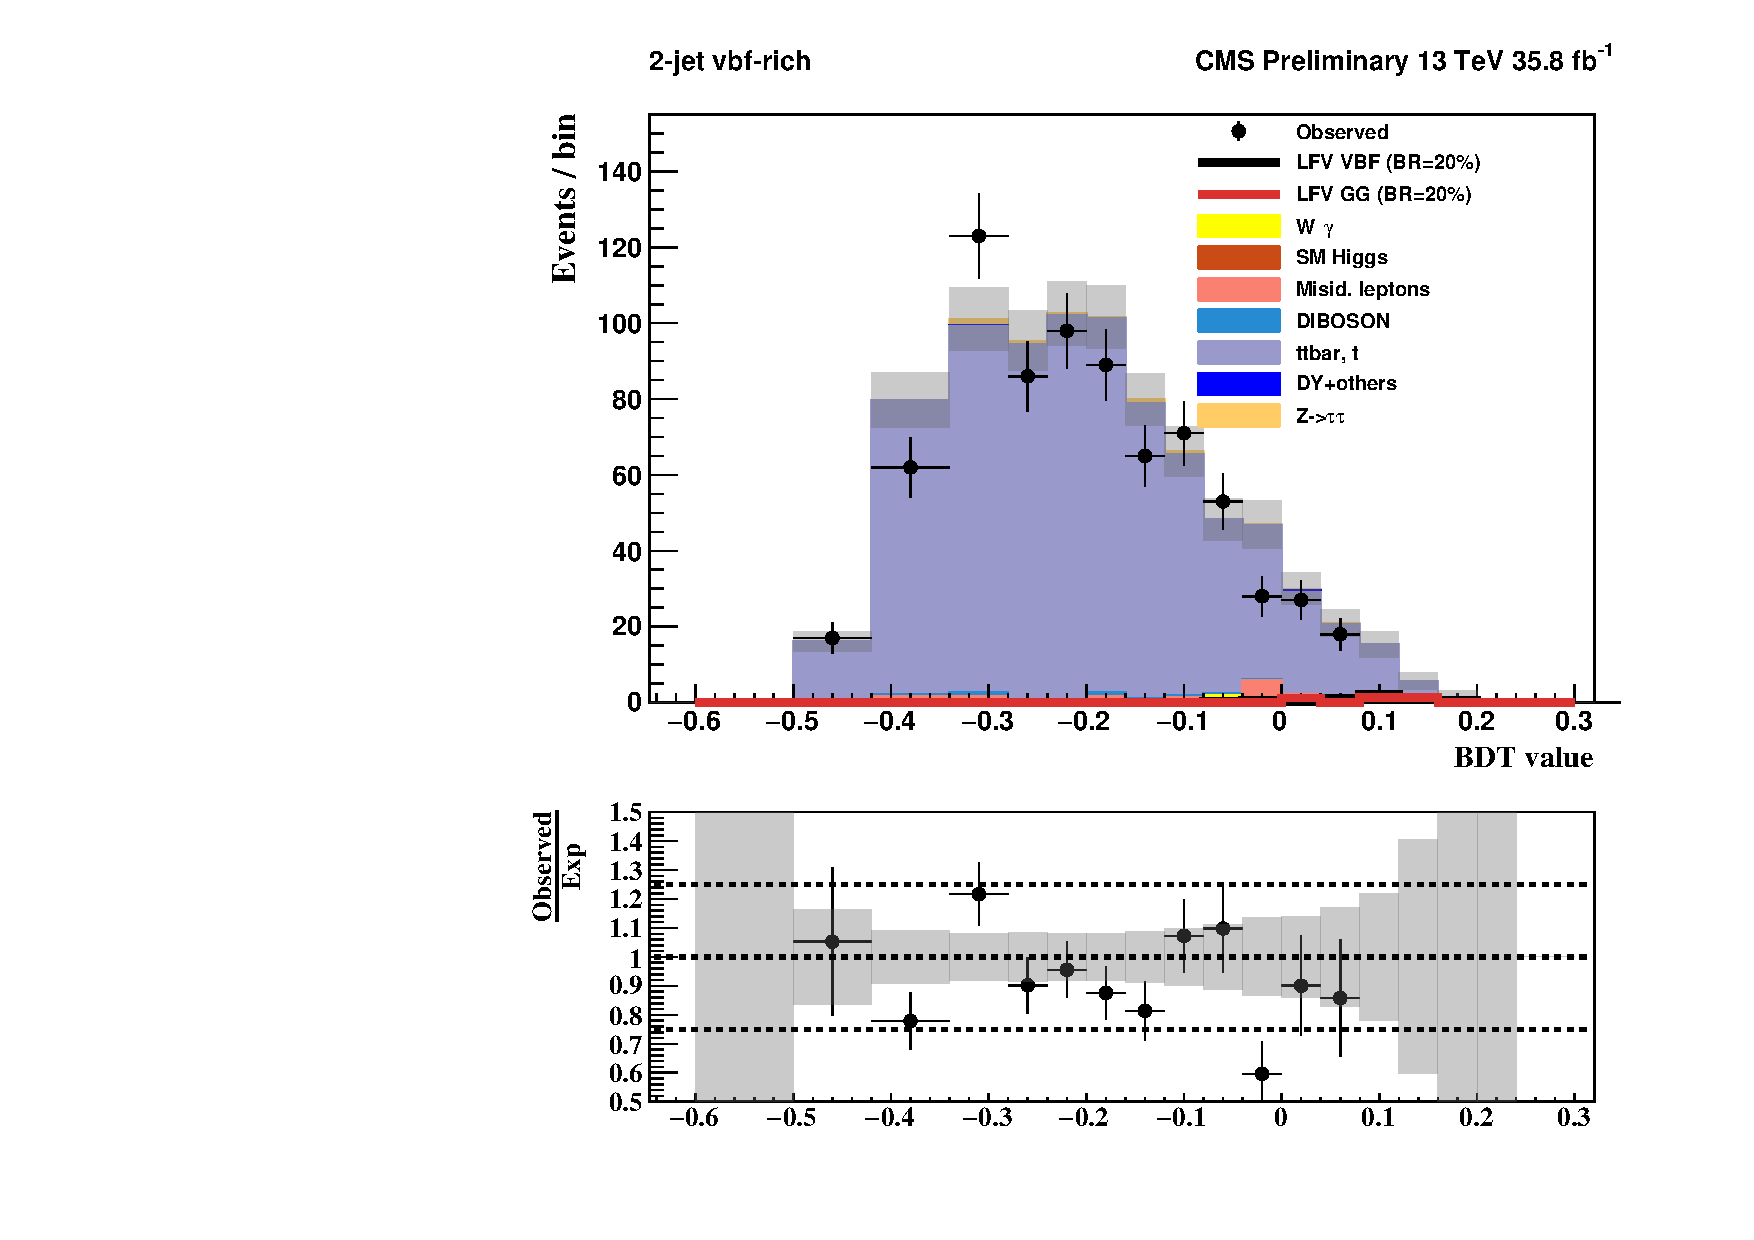
\includegraphics[width=0.30\textwidth]{plots_and_figures/chapter6/tt_cr/22_preselection_BDT_value.pdf} \\
 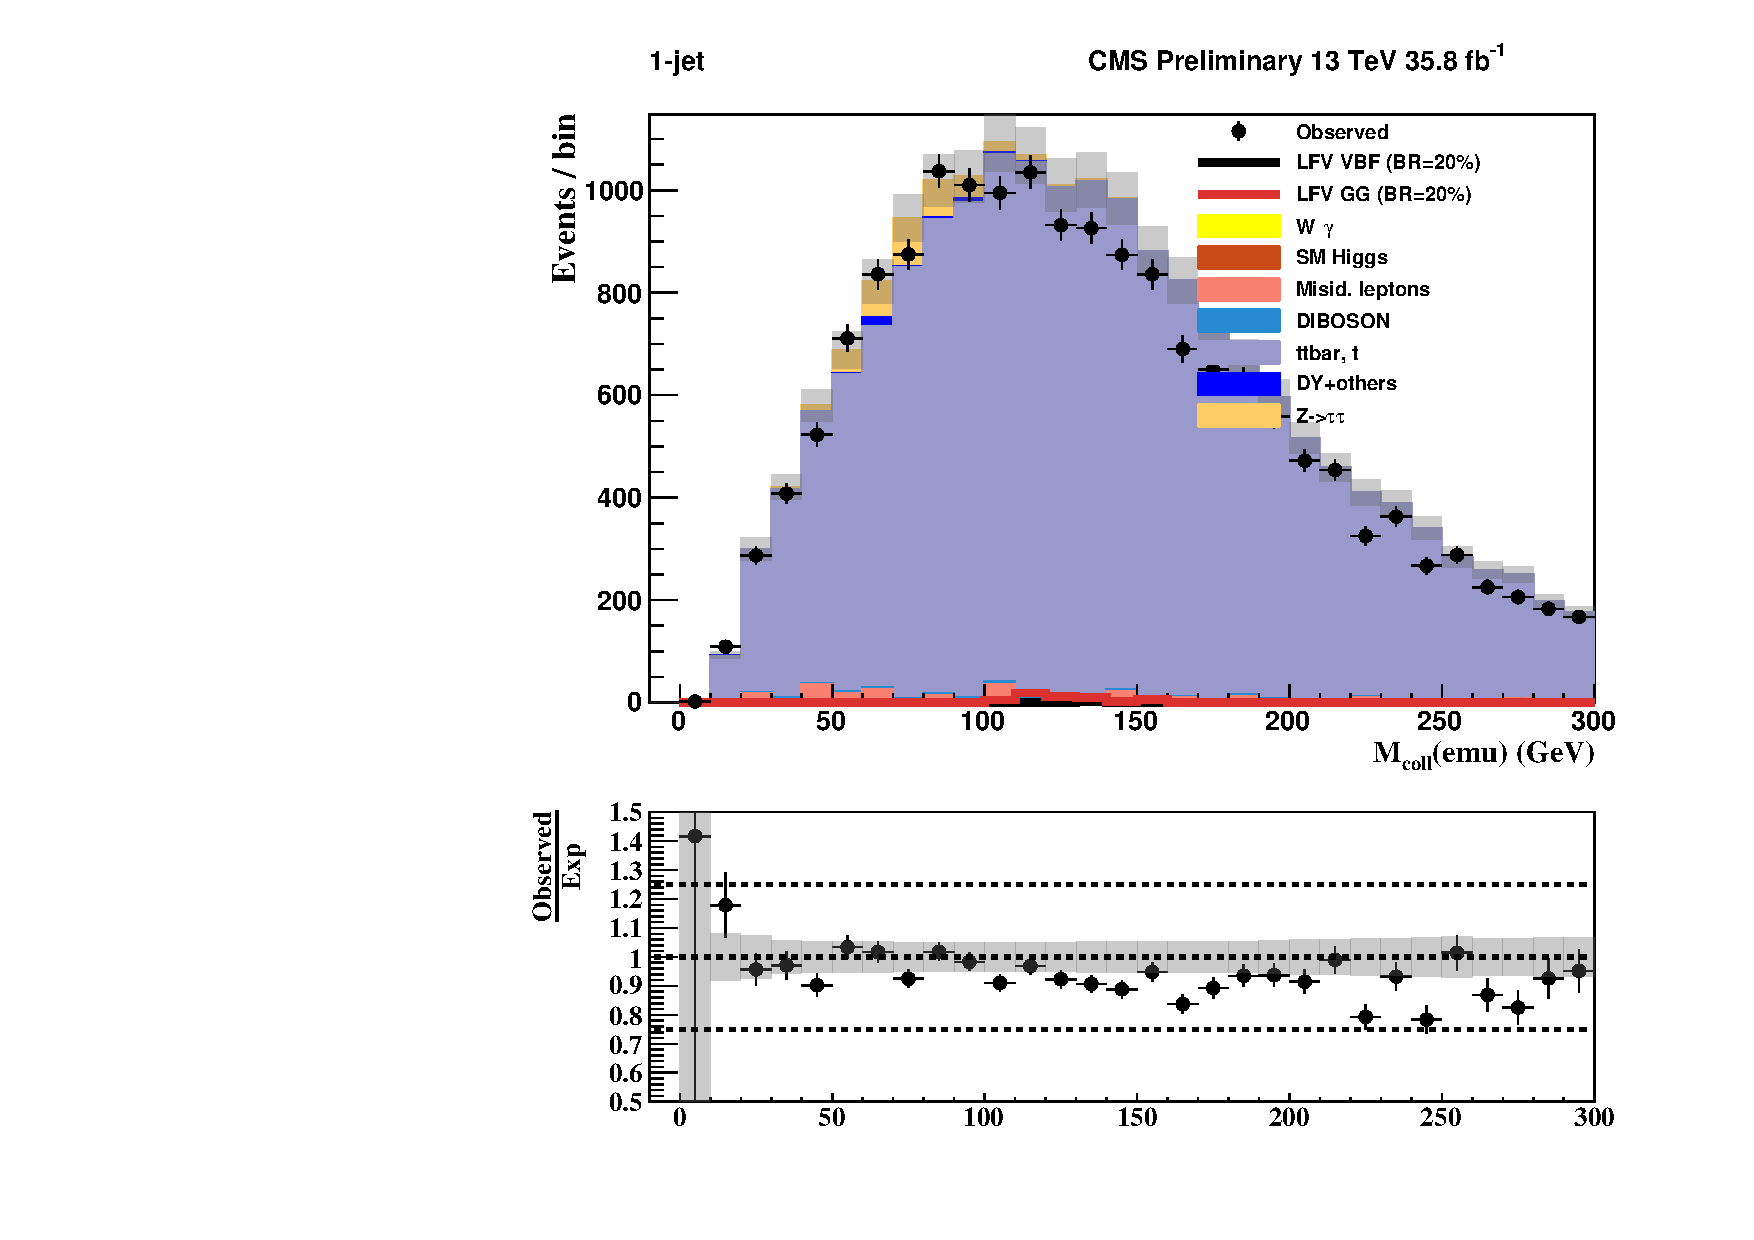
\includegraphics[width=0.30\textwidth]{plots_and_figures/chapter6/tt_cr/1_preselection_h_collmass_pfmet.pdf}
 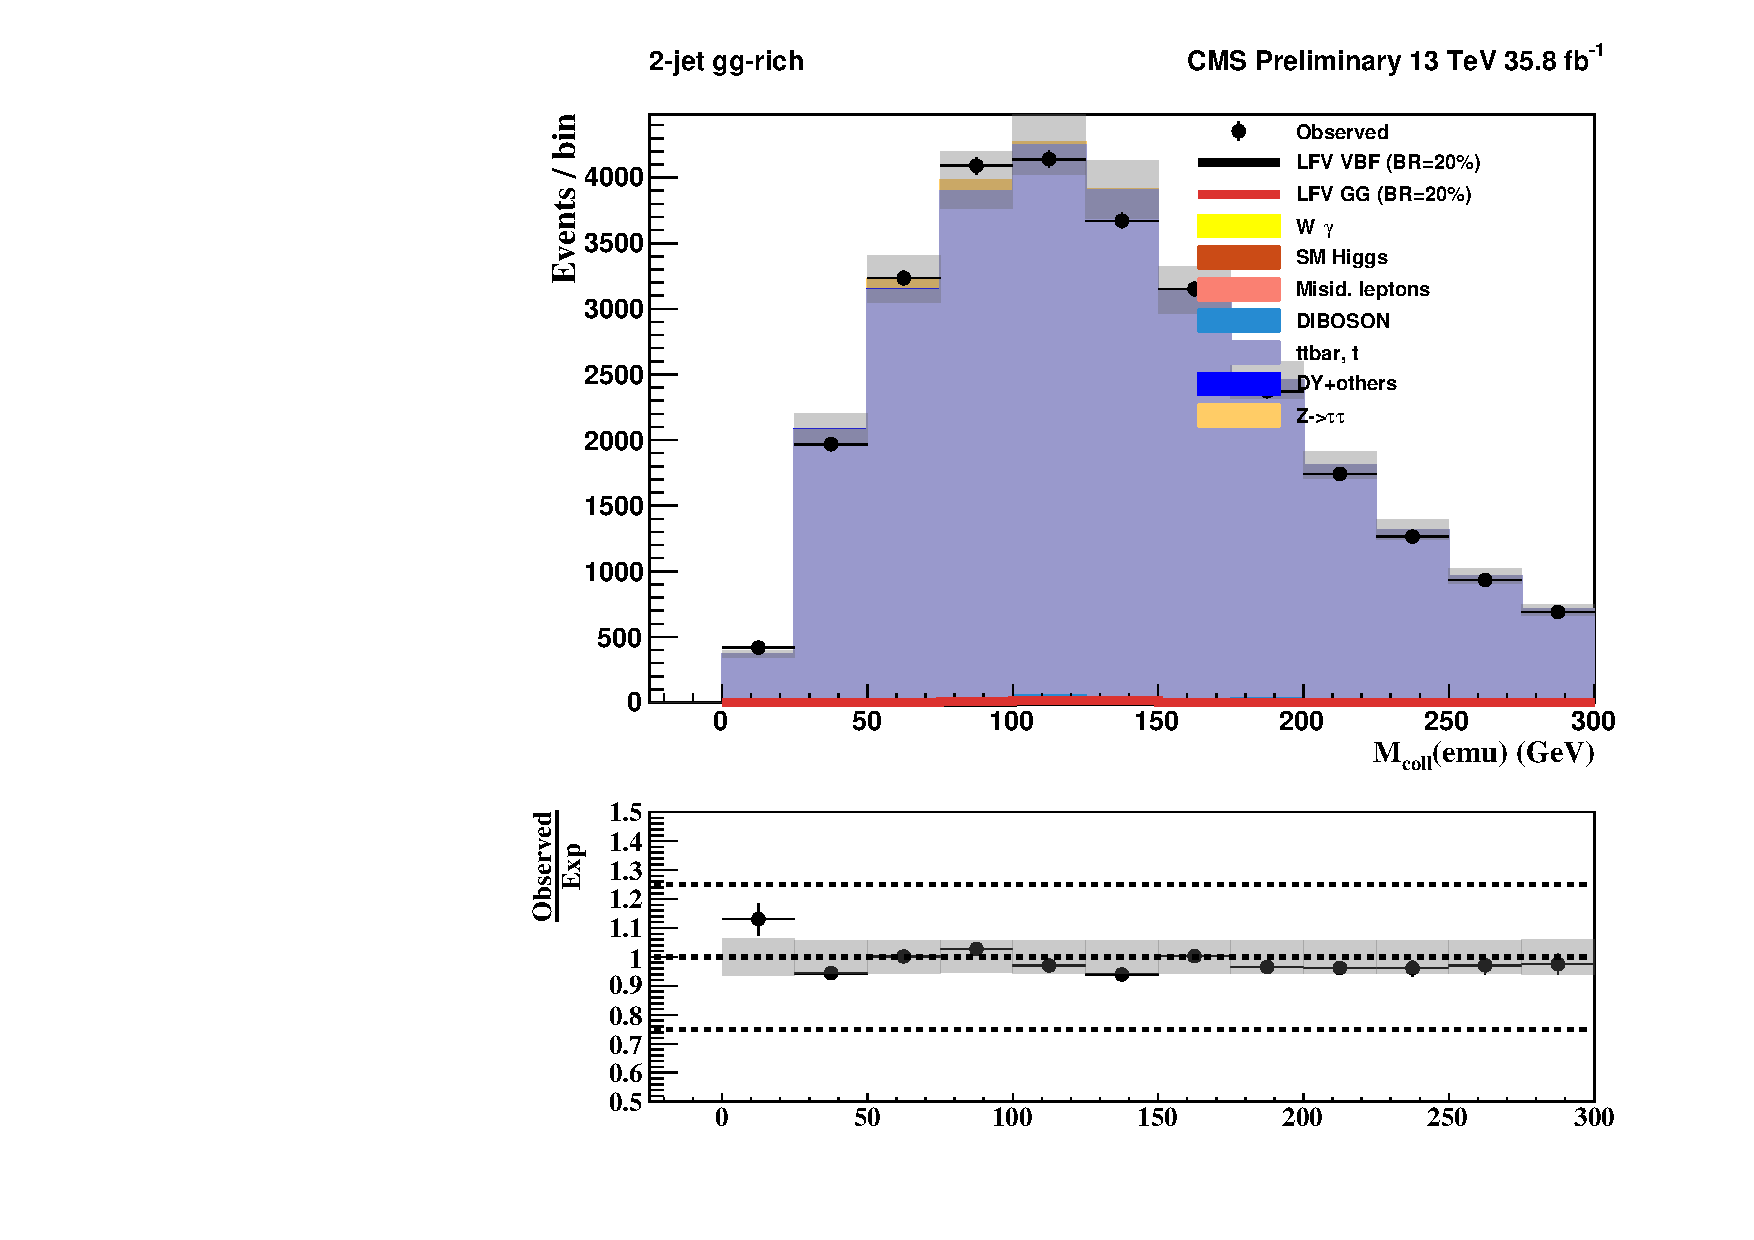
\includegraphics[width=0.30\textwidth]{plots_and_figures/chapter6/tt_cr/21_preselection_h_collmass_pfmet.pdf} 
 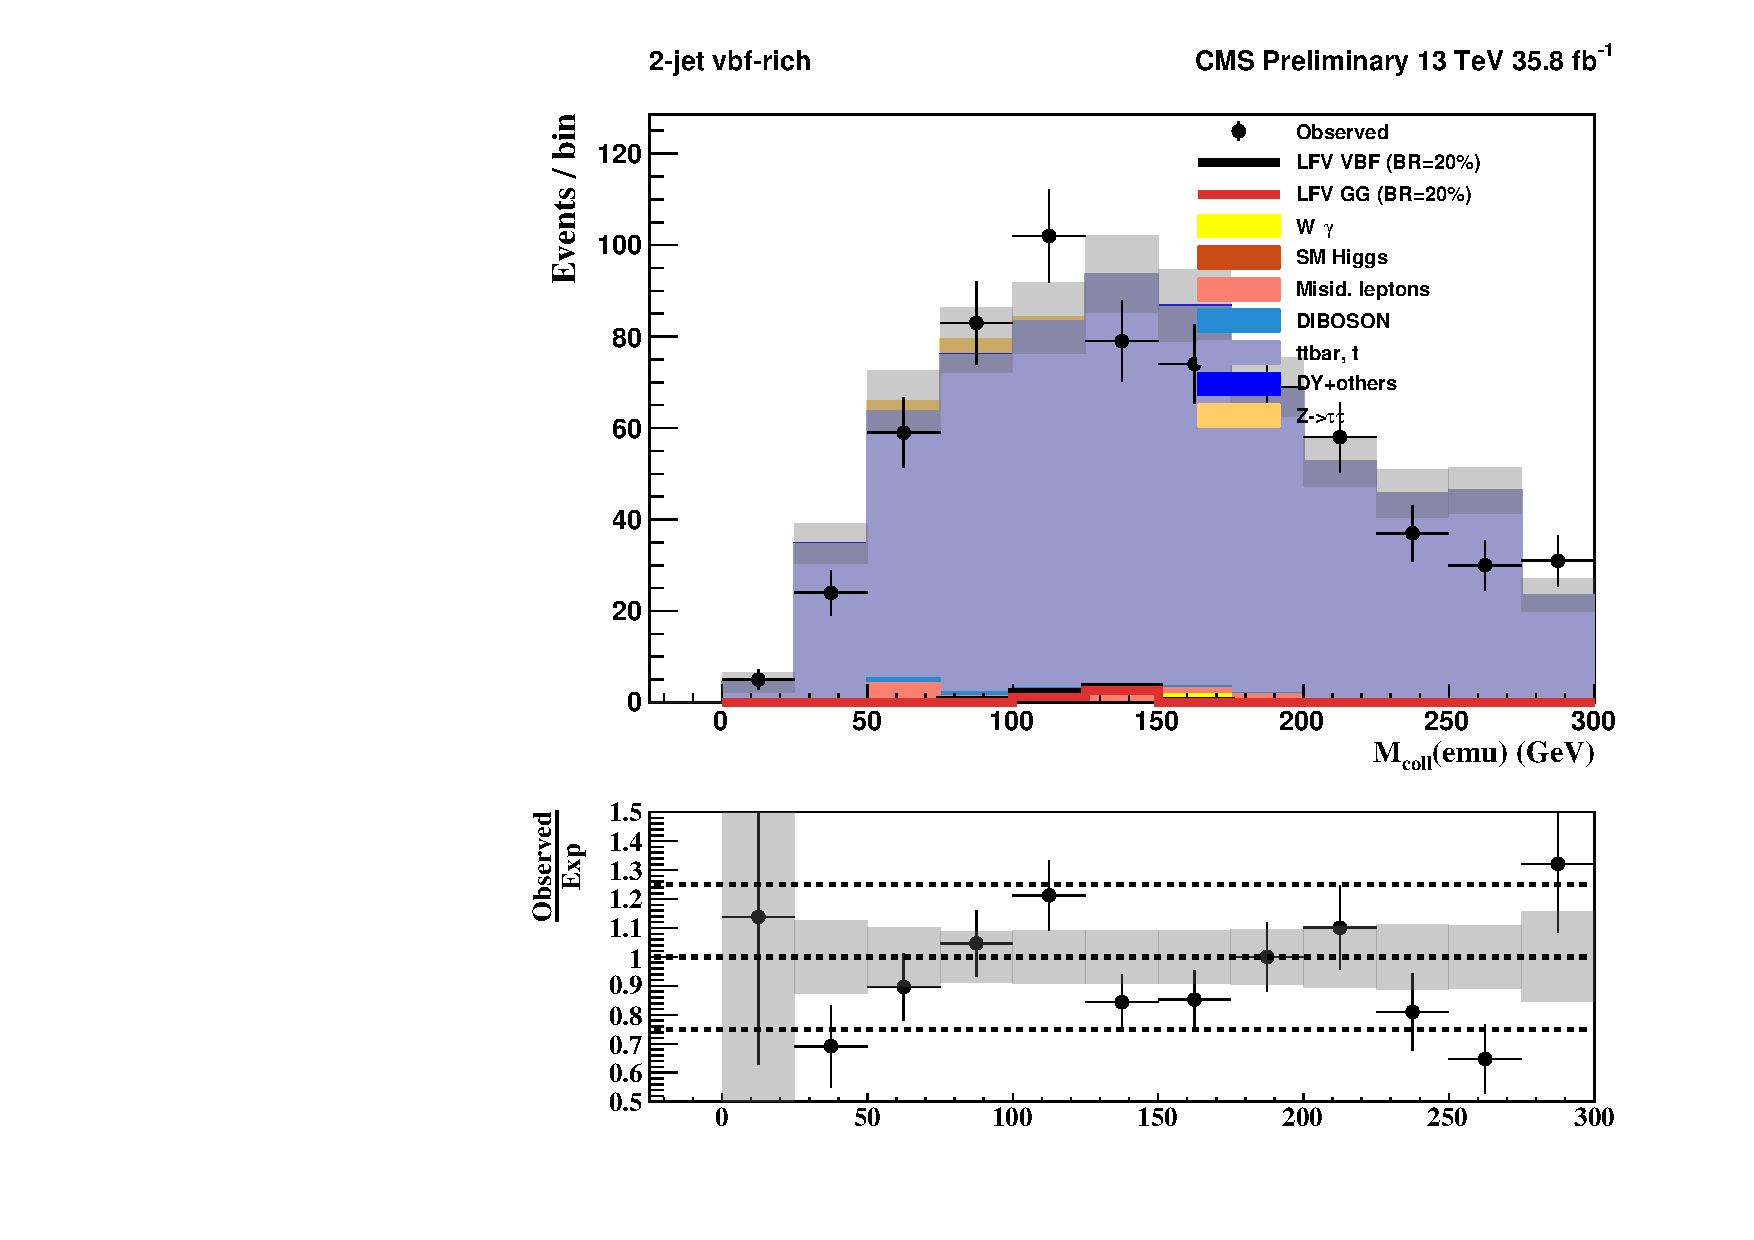
\includegraphics[width=0.30\textwidth]{plots_and_figures/chapter6/tt_cr/22_preselection_h_collmass_pfmet.pdf} \\


 \caption{Distributions of BDT response (top) an \mcol (bottom) in the first \ttb enriched region, as described in the text.}
 \label{fig:tt_cr}
\end{figure}

\begin{figure}[!htpb]\centering
 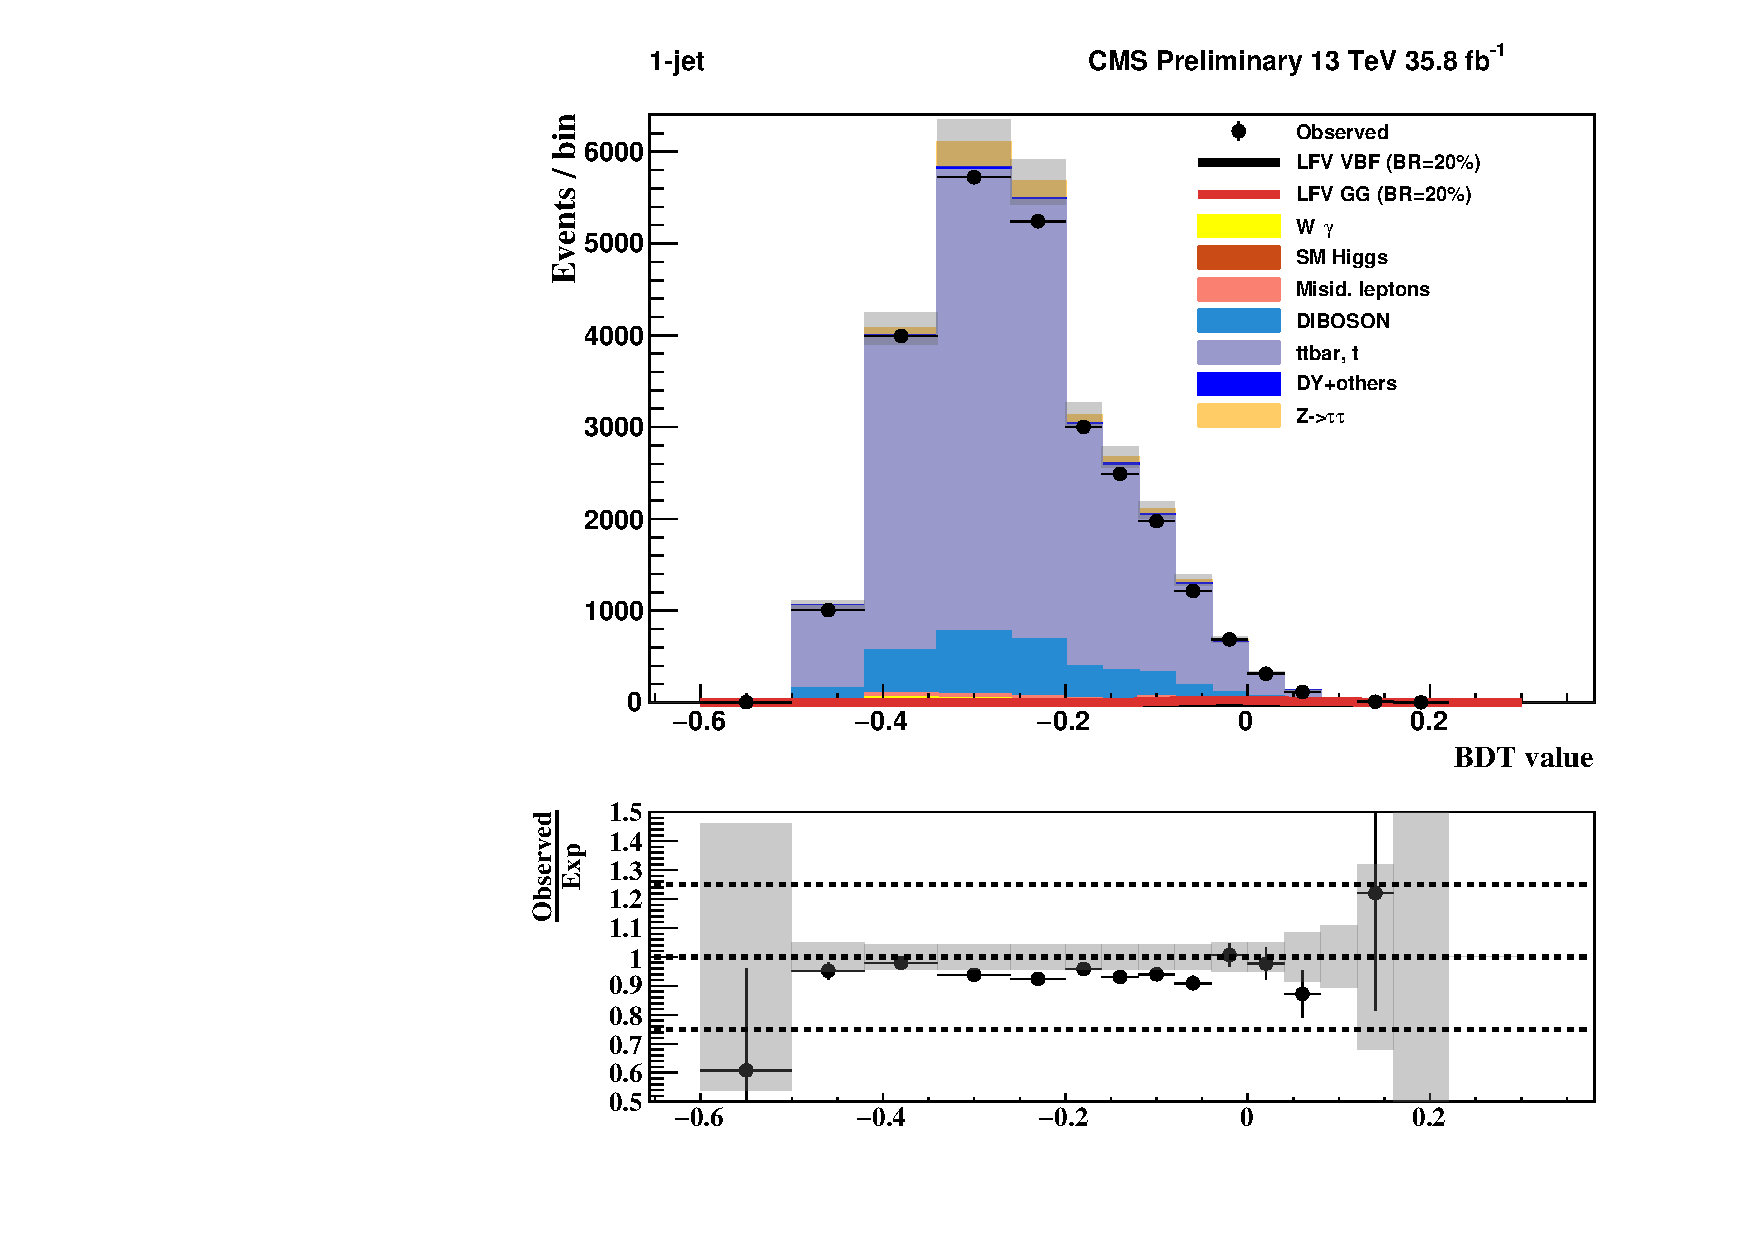
\includegraphics[width=0.30\textwidth]{plots_and_figures/chapter6/tt_cr_cutbased/1_preselection_BDT_value.pdf}
 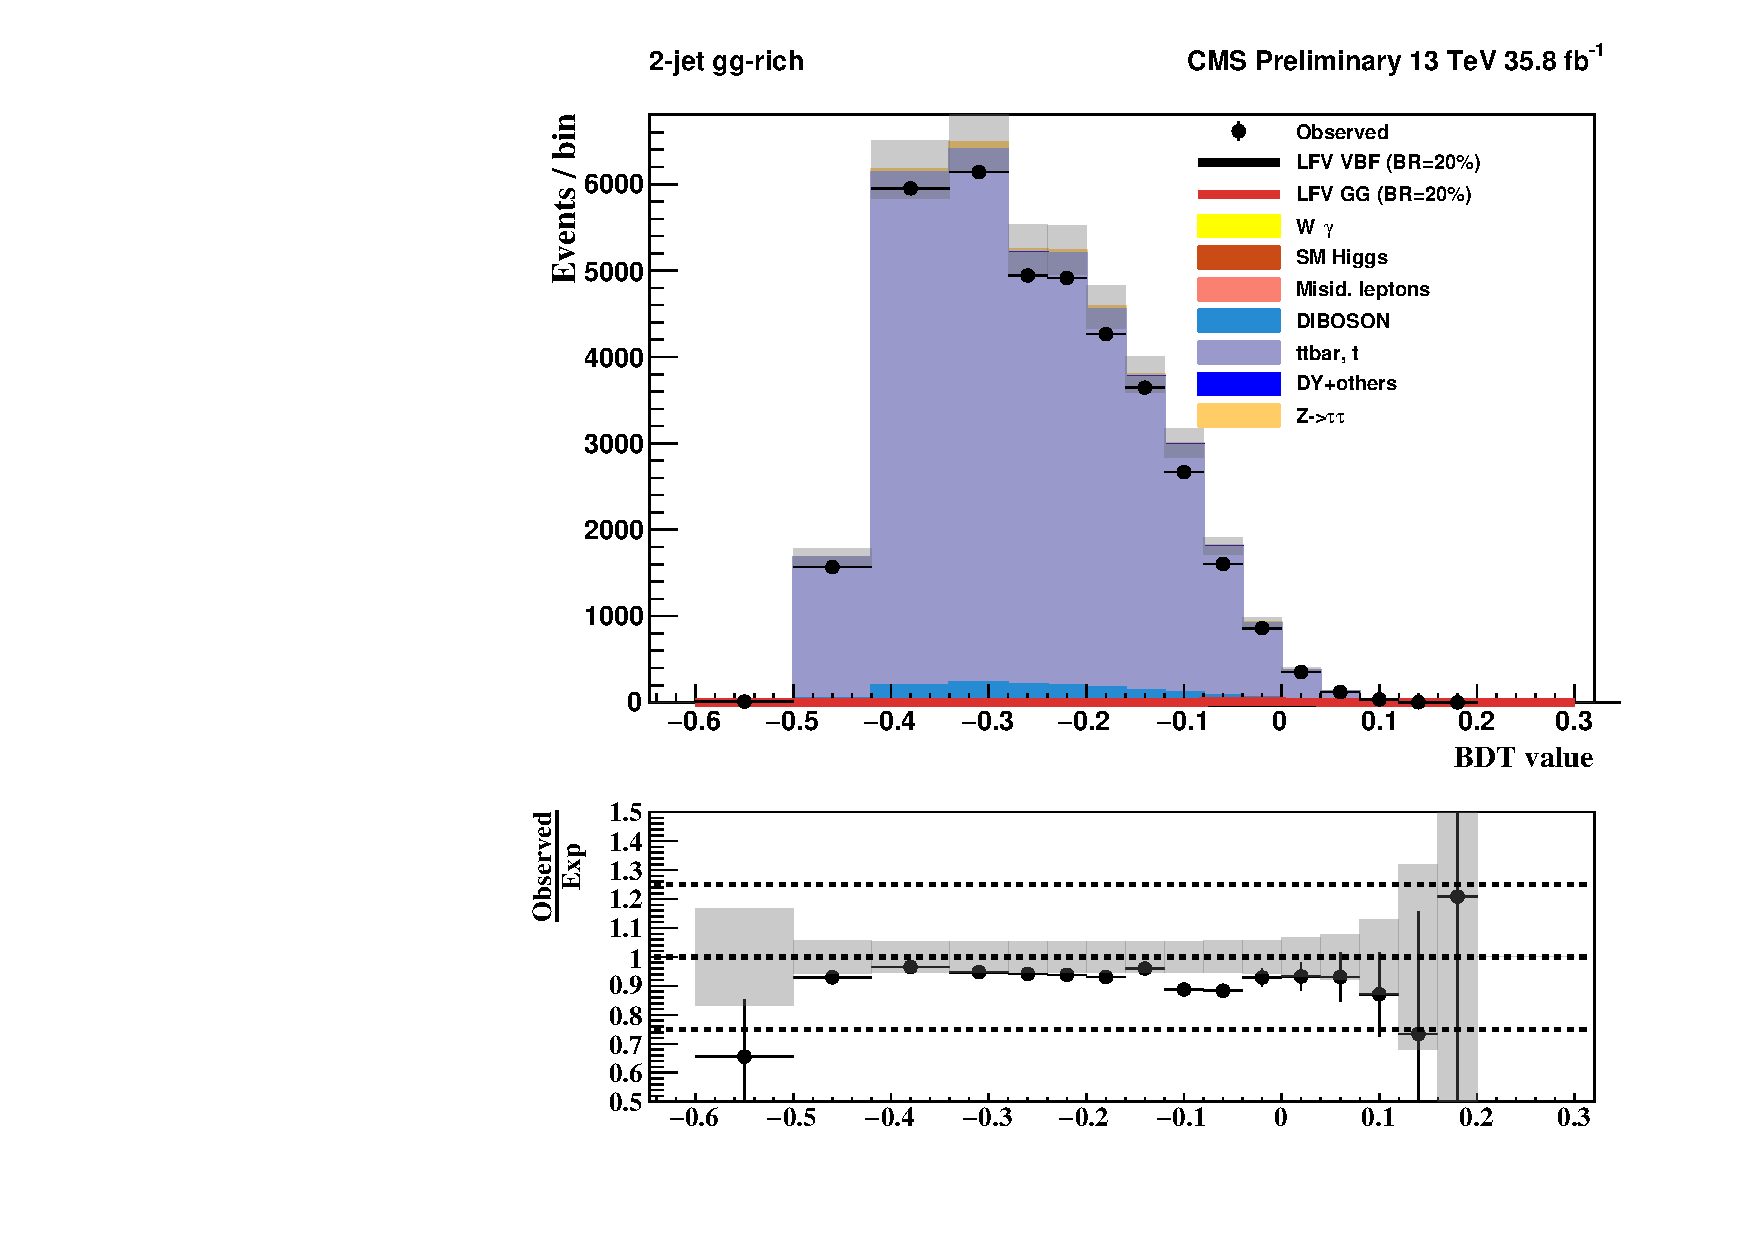
\includegraphics[width=0.30\textwidth]{plots_and_figures/chapter6/tt_cr_cutbased/21_preselection_BDT_value.pdf} 
 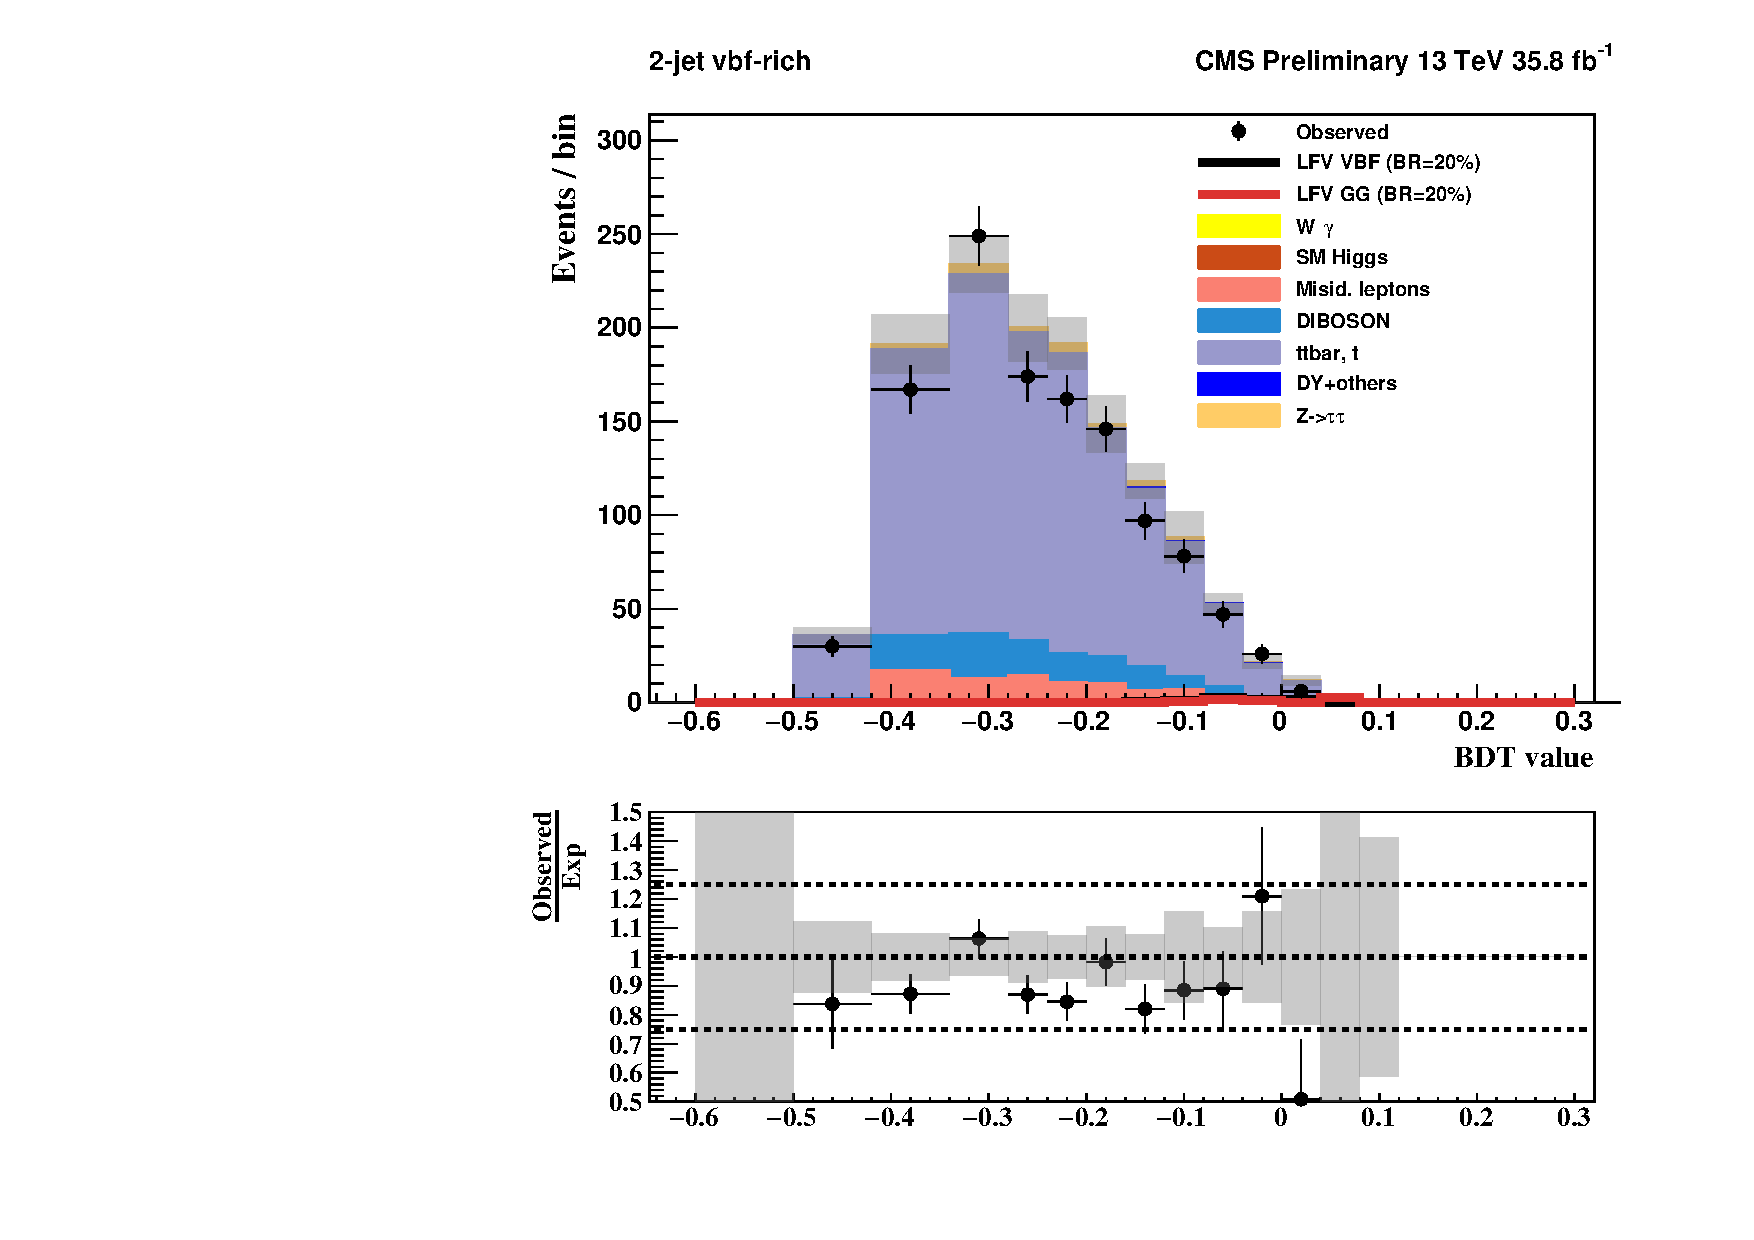
\includegraphics[width=0.30\textwidth]{plots_and_figures/chapter6/tt_cr_cutbased/22_preselection_BDT_value.pdf} \\
 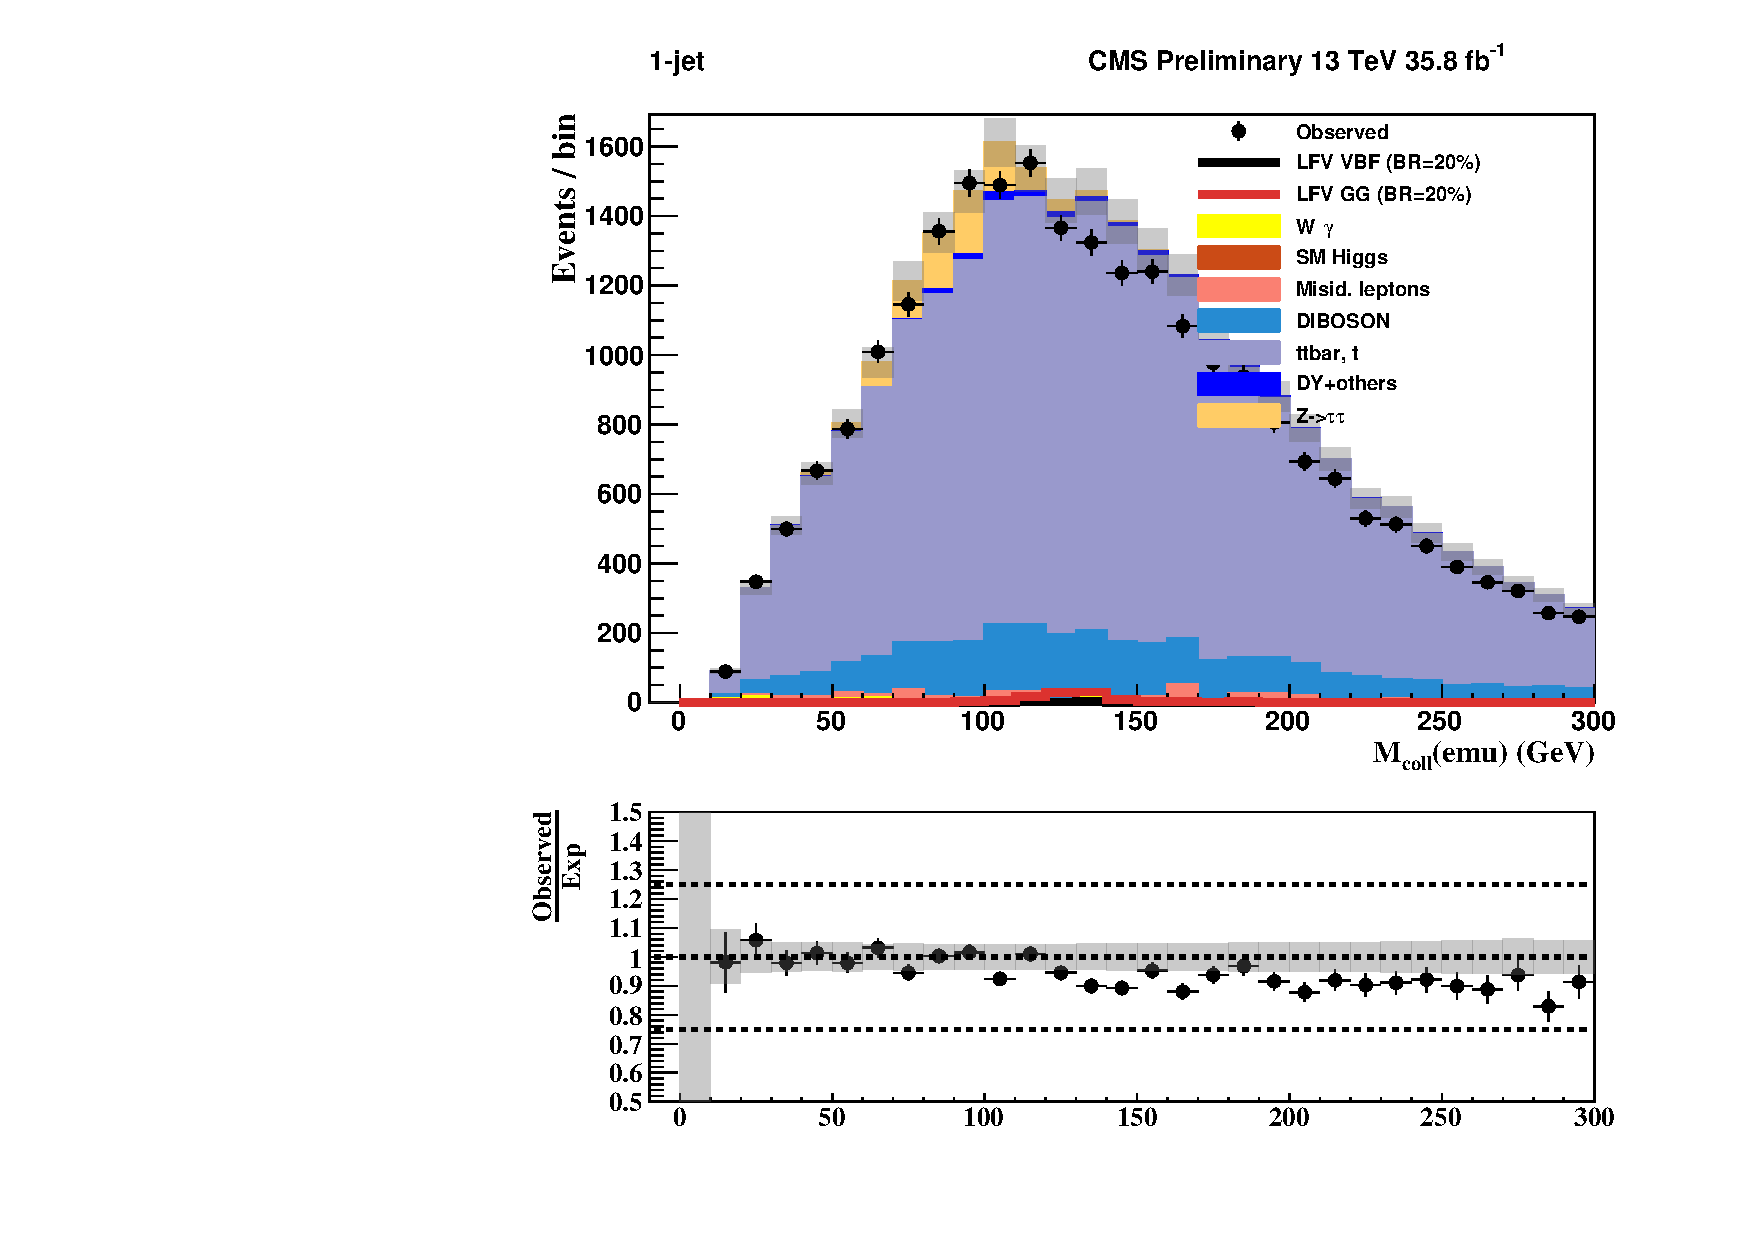
\includegraphics[width=0.30\textwidth]{plots_and_figures/chapter6/tt_cr_cutbased/1_preselection_h_collmass_pfmet.pdf}
 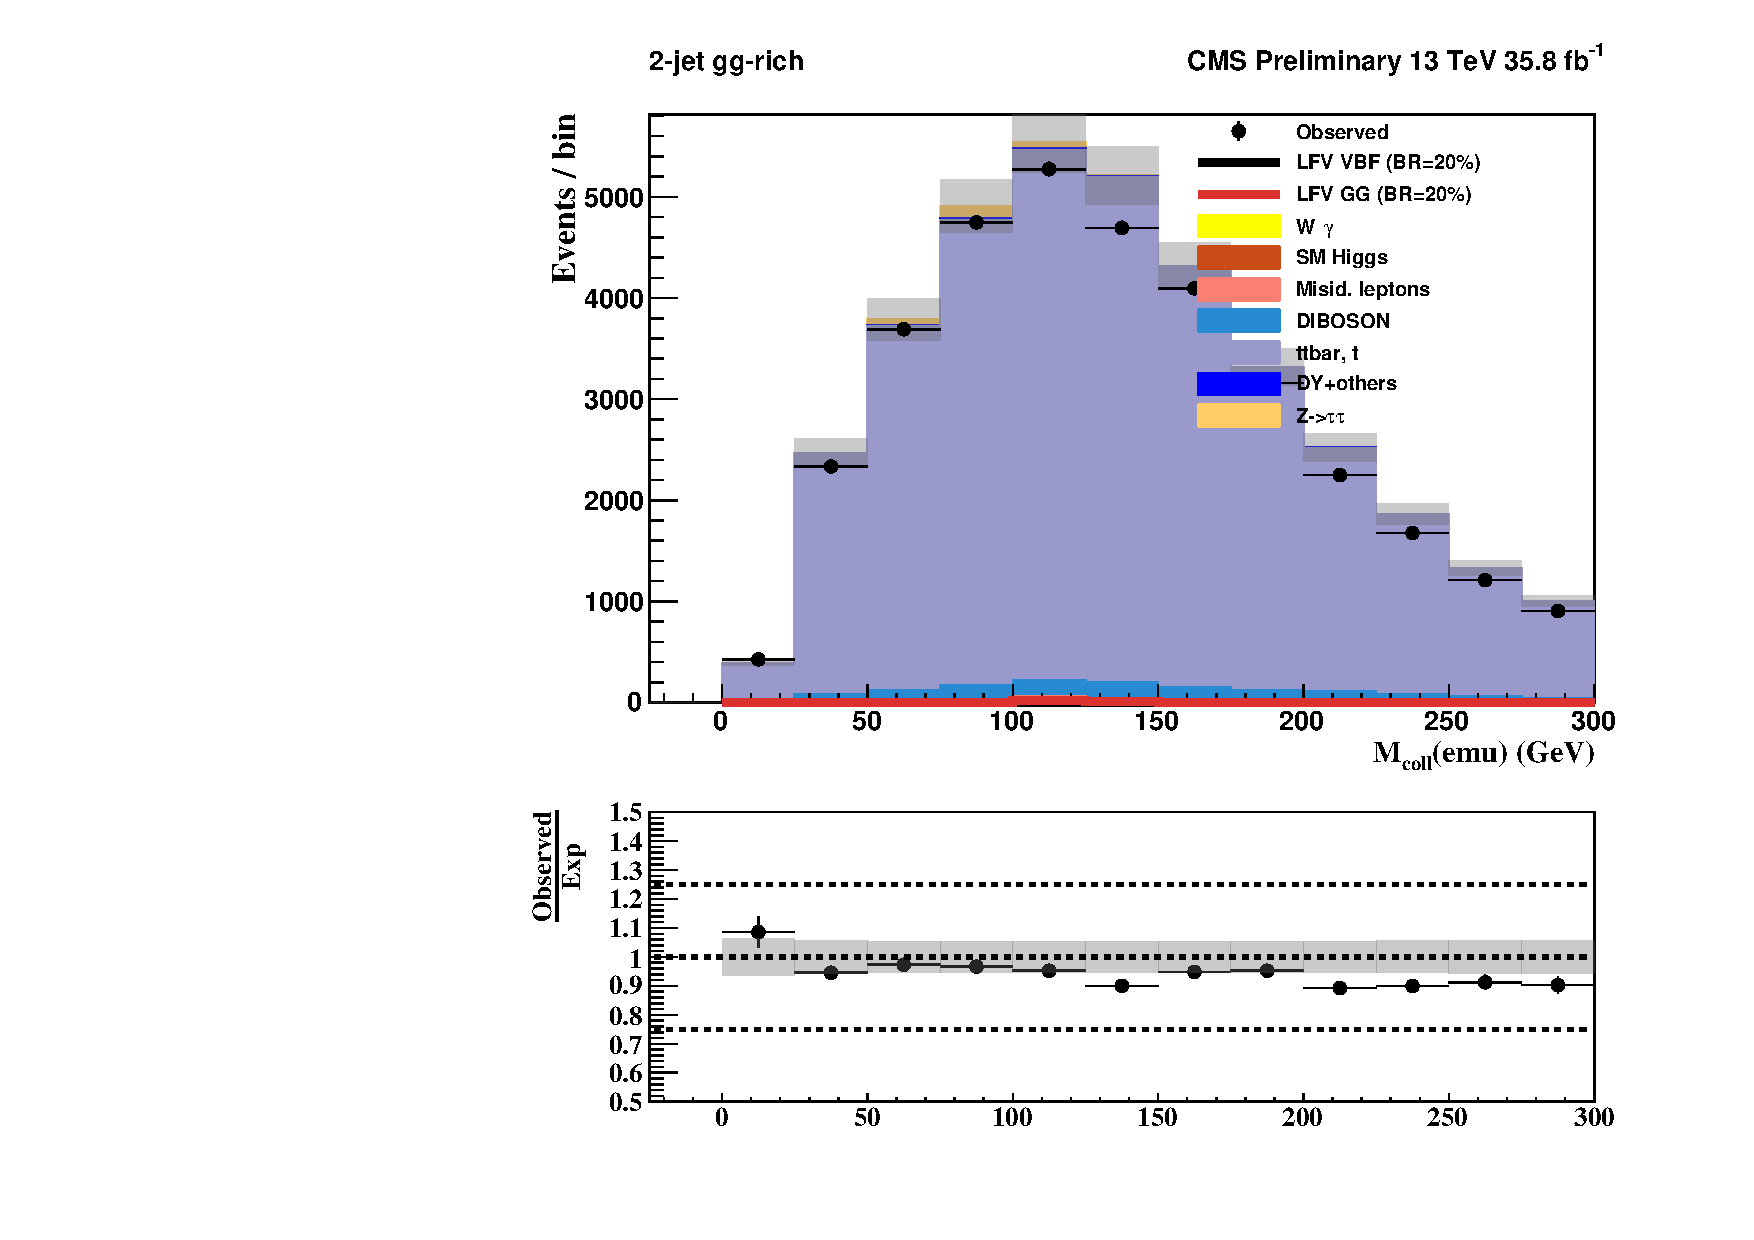
\includegraphics[width=0.30\textwidth]{plots_and_figures/chapter6/tt_cr_cutbased/21_preselection_h_collmass_pfmet.pdf} 
 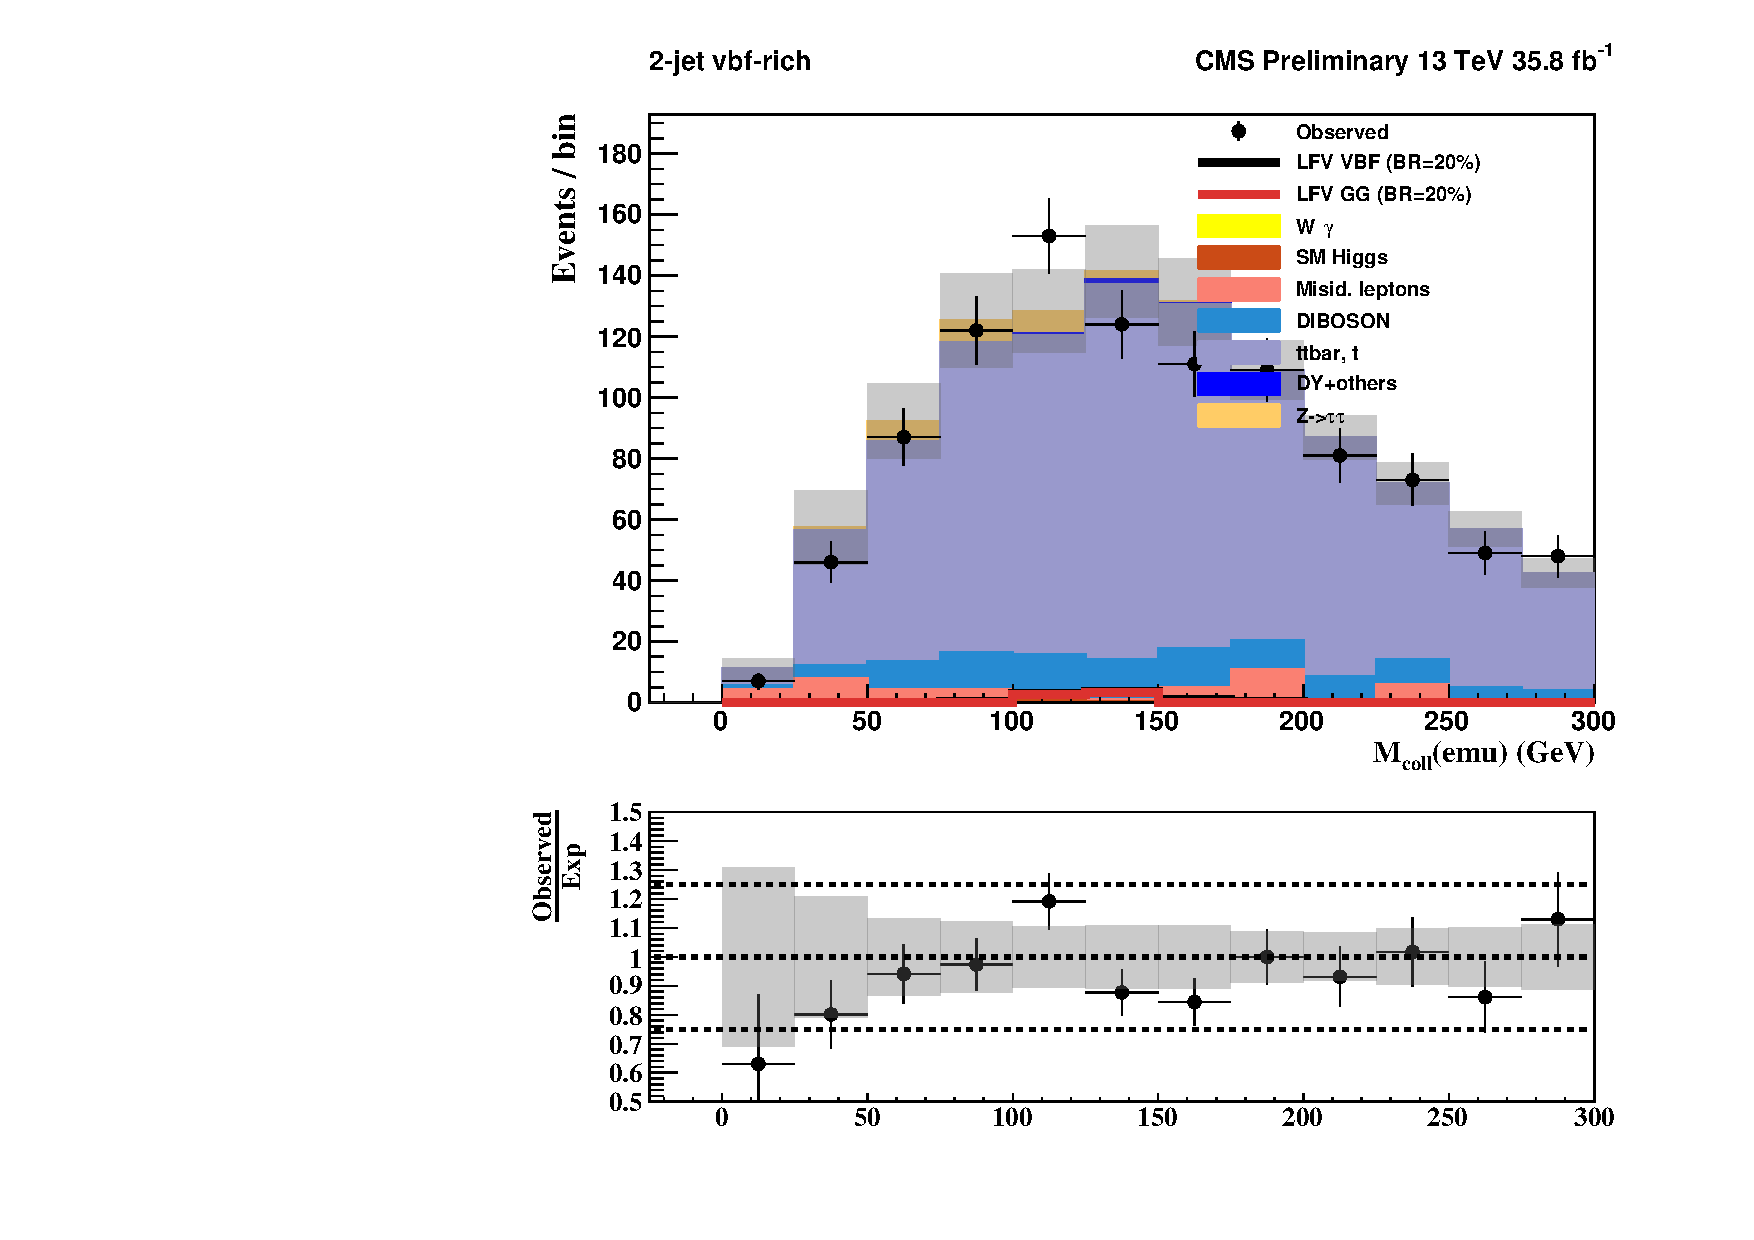
\includegraphics[width=0.30\textwidth]{plots_and_figures/chapter6/tt_cr_cutbased/22_preselection_h_collmass_pfmet.pdf} \\


 \caption{Distributions of BDT response (top) an \mcol (bottom) in the second \ttb enriched region, as described in the text.}
 \label{fig:tt_cr_cutbased}
\end{figure}

\subsection{Misidentified lepton background}
Another source of background which is relatively much smaller than \ttb or \ztt arises from jets misidentified as leptons in \wjets or SM events comprised uniquely of jets produced through the strong interaction, referred to as quantum chromodynamics (QCD) multijet events. In \wjets events one lepton candidate is a real lepton from the $\PW$ boson decay while the other lepton is a misidentified jet. In QCD events, both leptons in the final state are misidentified jets. The baseline selection criteria requires the leptons to be well identified and isolated. This makes it difficult for a jet to masquerade as a lepton. In case of the $\Pgm$ this even more so since it is required to satisfy high $\pt$ thresholds as well. Consequently, these events form a small part of the background. This is in contrast to a final state where the non-prompt lepton is a hadronically decaying $\Pgt$ instead of an electronically decaying one. This background would be much larger in such a case.

The W + jets background contribution to the misidentified-lepton background is estimated using simulation. The QCD multijet contribution is estimated from collision data events where the leptons have like-signcharge. The expected yield from non-QCD processes in this region is subtracted using simulation. The resulting sample is then rescaled to account for the differences between the composition in the like- and opposite-sign charge regions. The scaling factors are extracted from samples enriched  QCD multijet events, and the procedure is illustrated in Ref.~\cite{}. This background is validated in a control region that is obtained by requiring the baseline selection but inverting the isolation criteria. In other words events with well-isolated $\Pgm$ and $\Pe$ are rejected. The particular isolation thresholds required for this region are:$1>I_\text{rel}^{\Pe} > 0.1$ or $0.25>I_\text{rel}^{\Pgm} > 0.15$. The distributions of BDT response and \mcol in this qcd enriched region are shown in Fig.~\ref{fig:qcd_cr}. The plots show good agreement between data and background.



\begin{figure*}[!htpb]\centering
 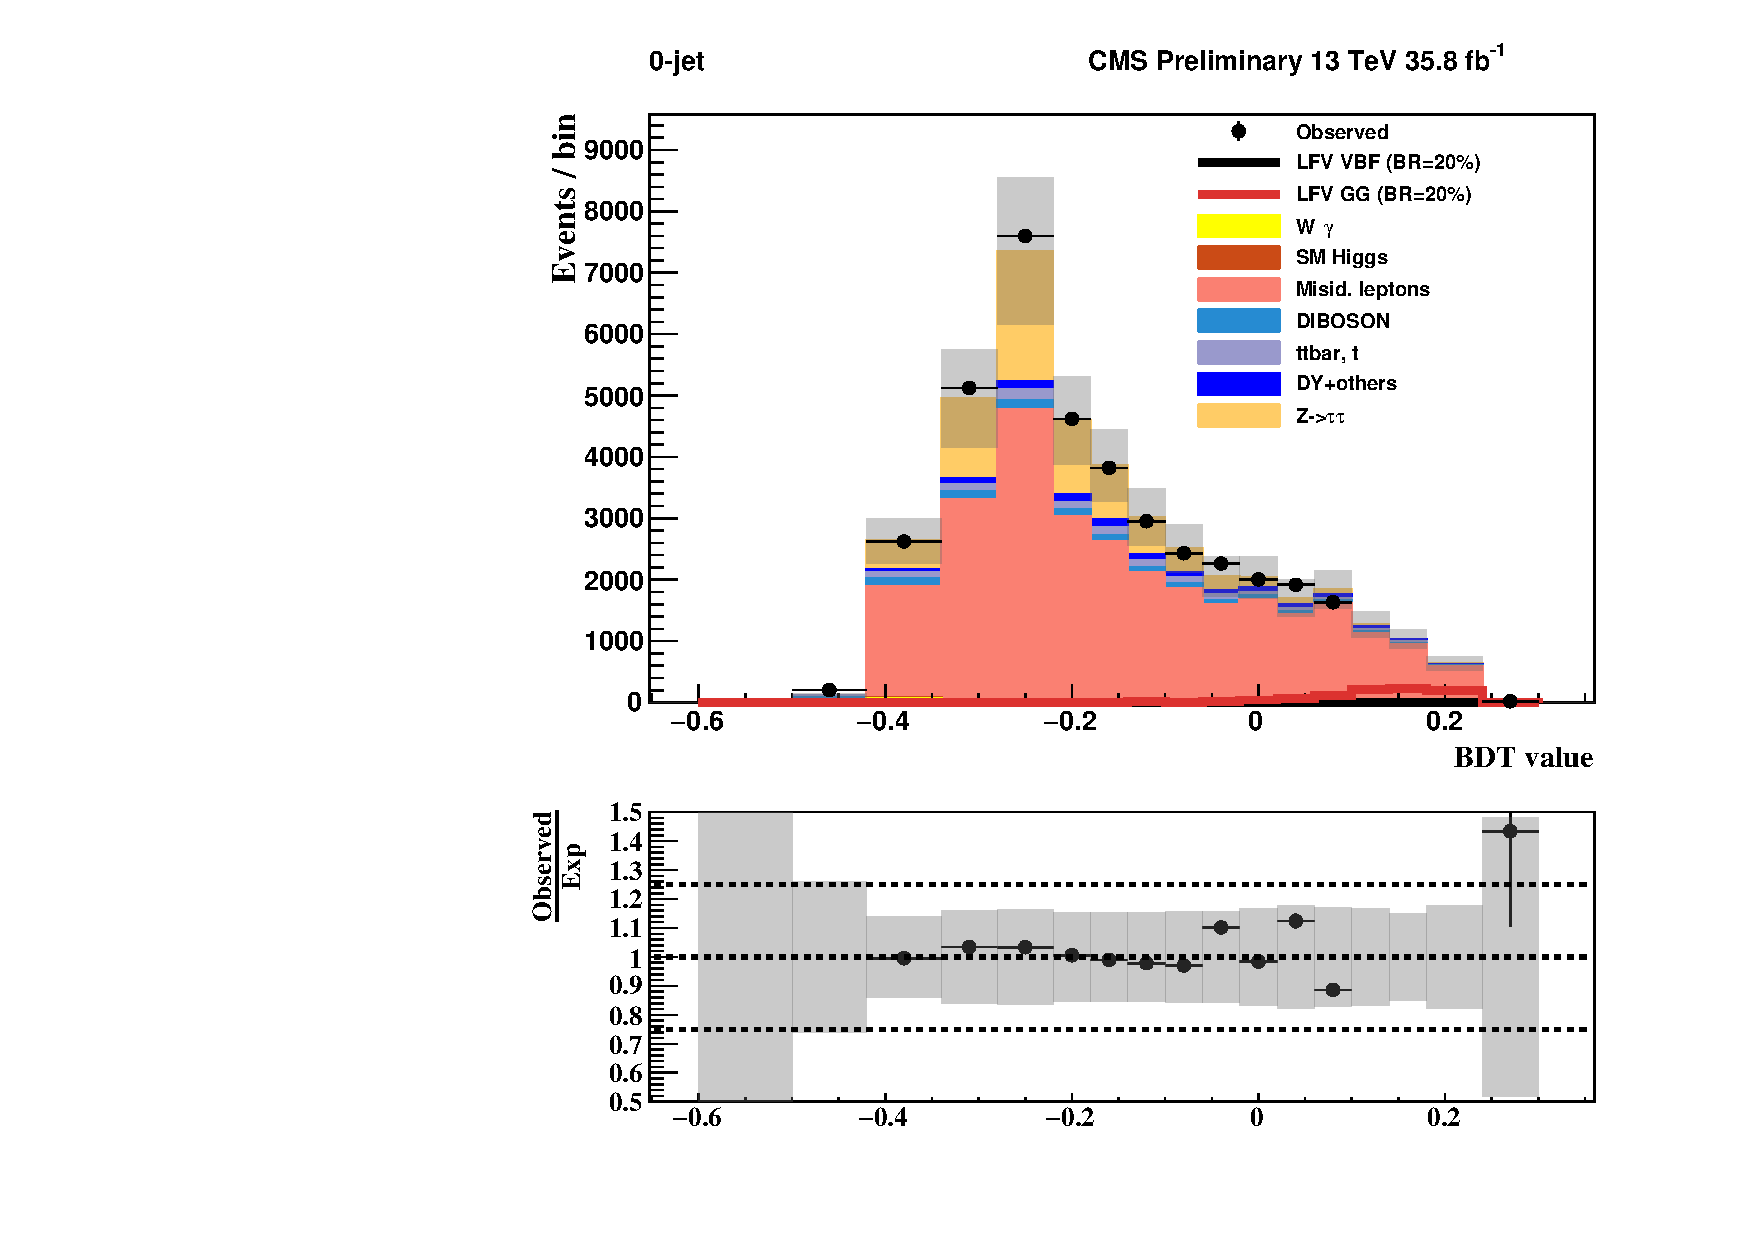
\includegraphics[width=0.49\textwidth]{plots_and_figures/chapter6/qcd_cr/0_preselection_BDT_value.pdf}
 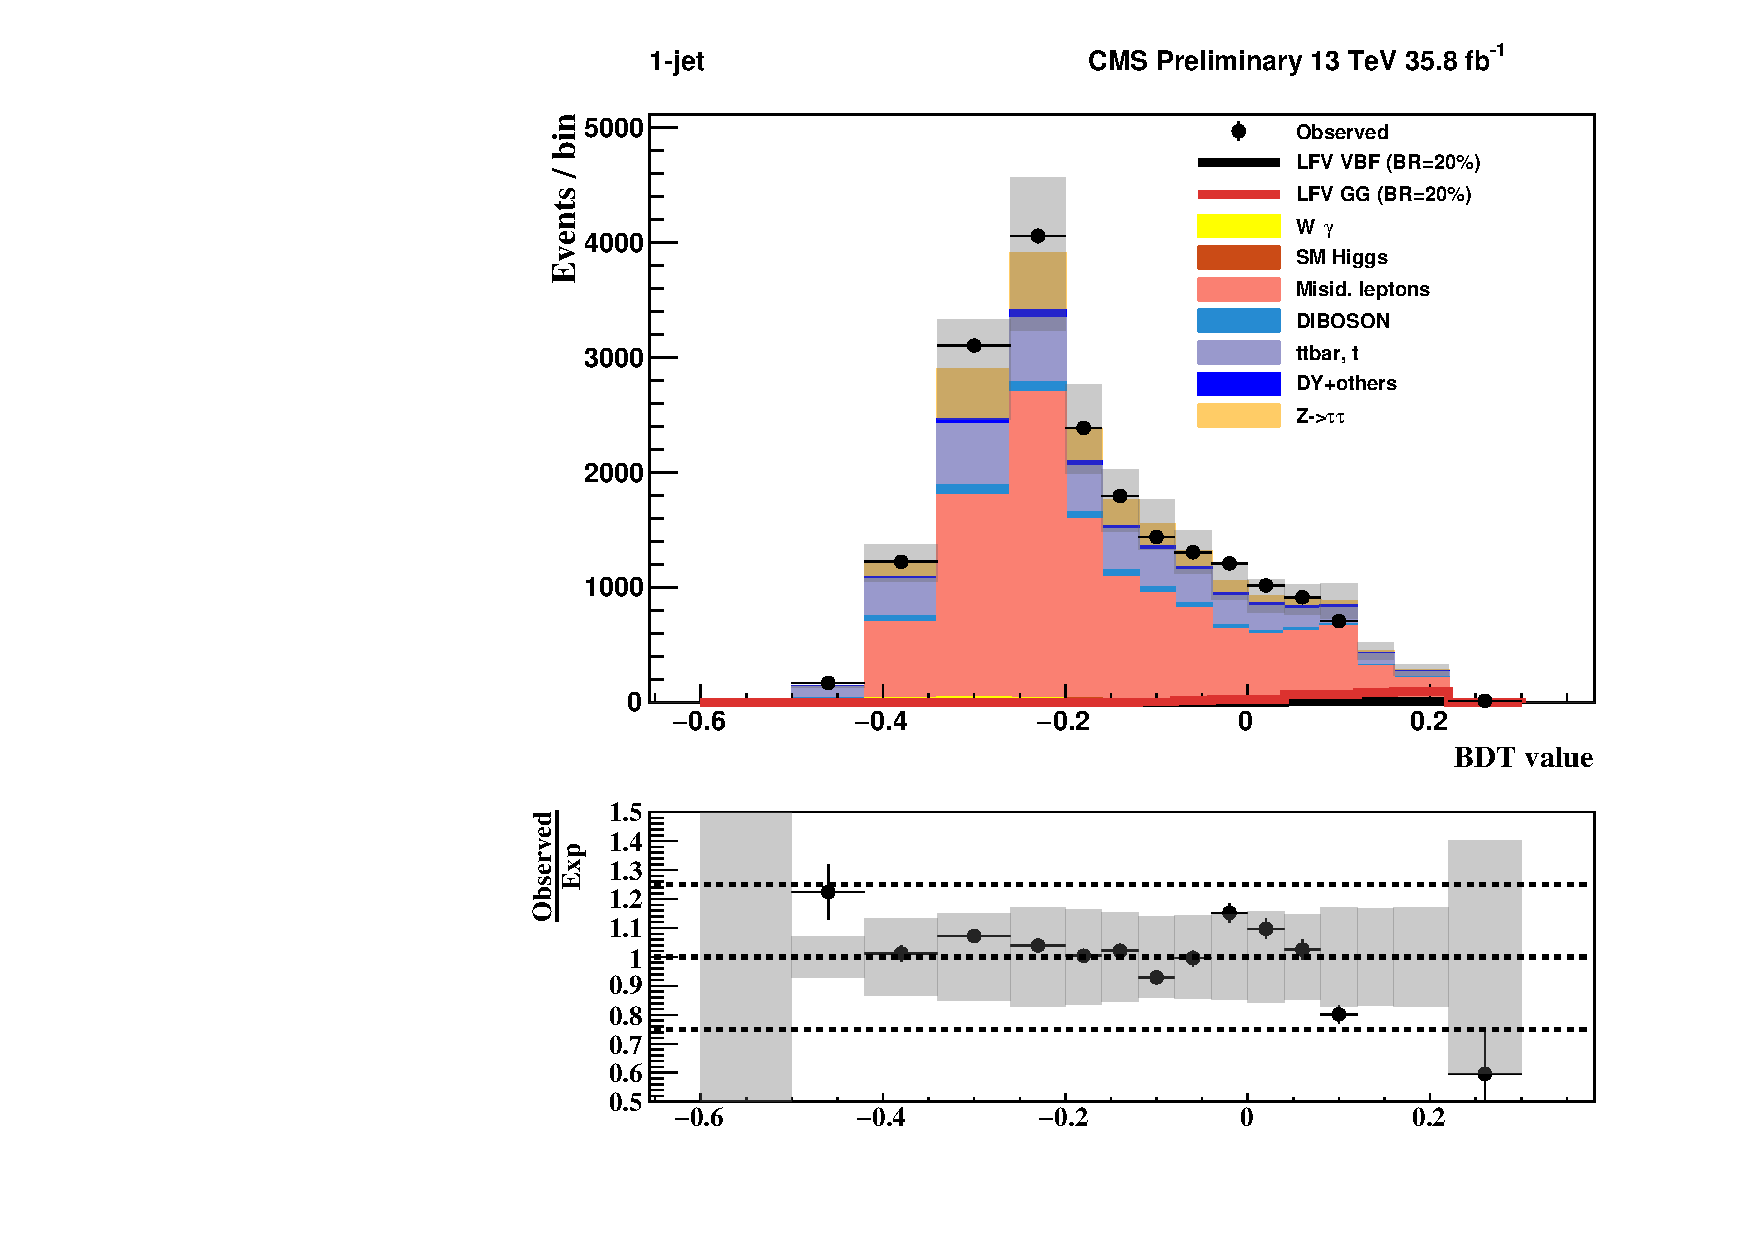
\includegraphics[width=0.49\textwidth]{plots_and_figures/chapter6/qcd_cr/1_preselection_BDT_value.pdf} \\
 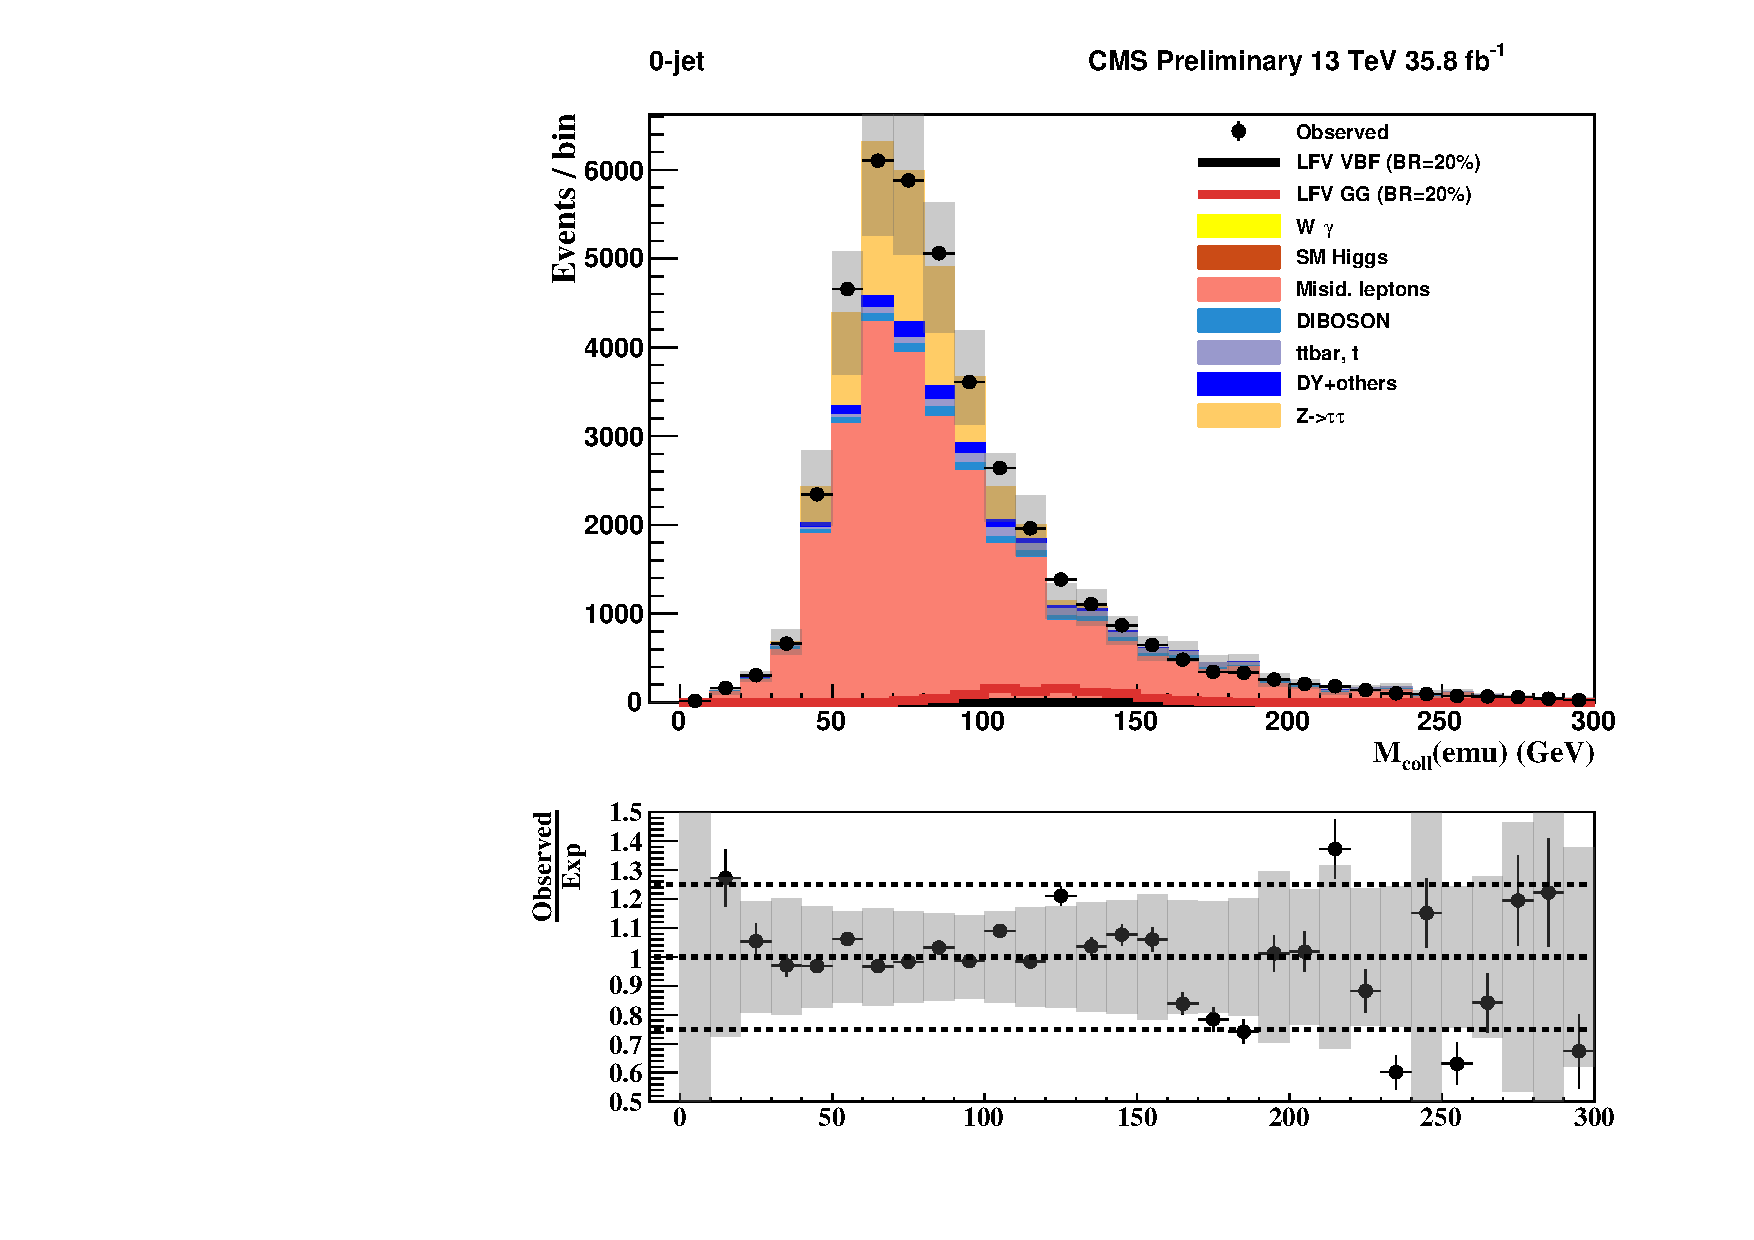
\includegraphics[width=0.49\textwidth]{plots_and_figures/chapter6/qcd_cr/0_preselection_h_collmass_pfmet.pdf} 
 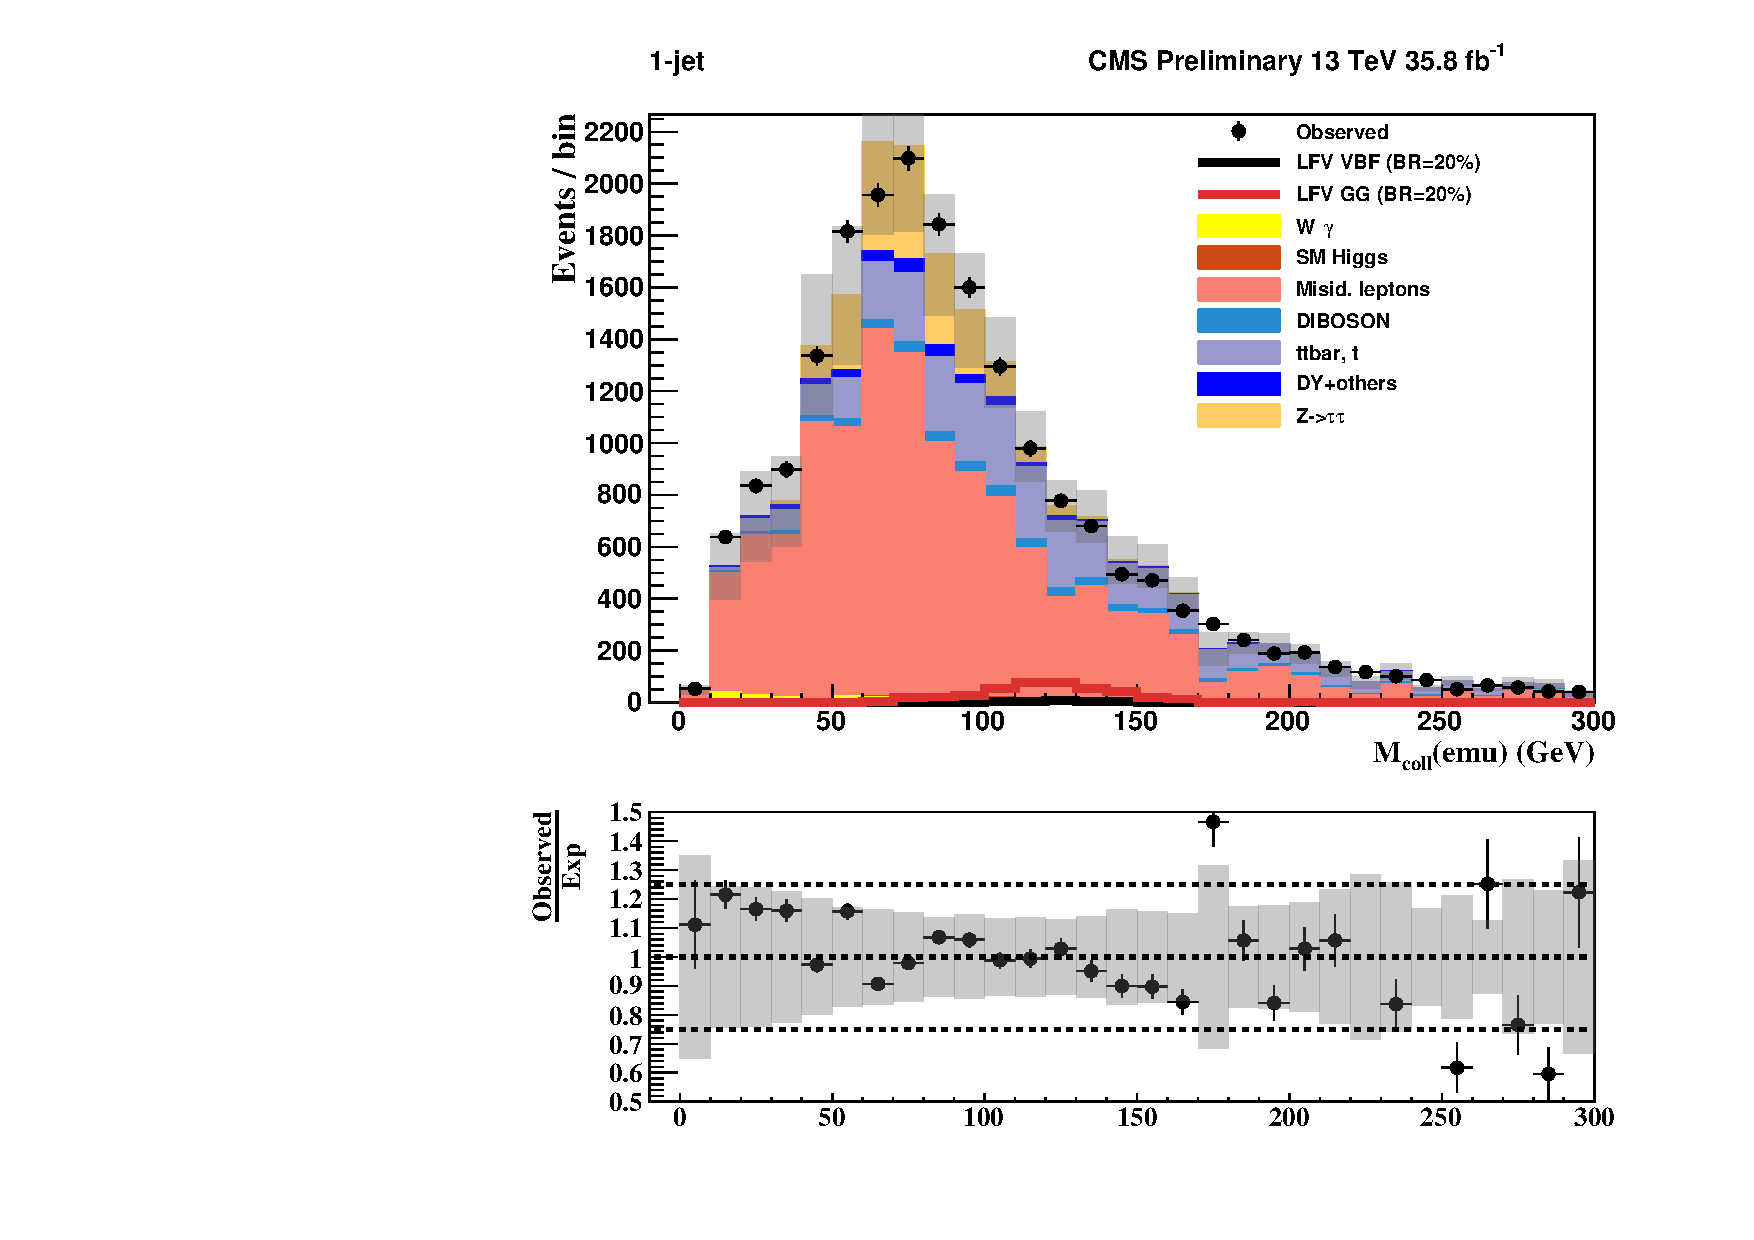
\includegraphics[width=0.49\textwidth]{plots_and_figures/chapter6/qcd_cr/1_preselection_h_collmass_pfmet.pdf} \\

 \caption{Distributions of BDT response (top) an \mcol (bottom) in QCD enriched region for 0-jet (left)  and 1-jet (right) categories.}
 \label{fig:qcd_cr}
\end{figure*}

\subsection{Other backgrounds}
The other backgrounds in the analysis make relatively much smaller contrbutions. Electroweak diboson production ($\PW\PW$, $\PW\PZ$ and $\PZ\PZ$) contributes a similar number of events as the misidentified lepton background. $\PW\PW$ events make the largest contribution, followed by $\PW\PZ$ and $\PZ\PZ$ events as the latter ones have additional leptons in their final state. SM decays of the h boson forms a small but non-negligible background. These come from $\text{h} \to \Pgt\Pgt$  and $\text{h} \to \PW\PW$ decays.

\section{Heavy Higgs Analysis}
\label{hh_bg_val}



% % uncomment the following lines,
% if using chapter-wise bibliography
%
% \bibliographystyle{ndnatbib}
% \bibliography{example}
